\documentclass[14pt, oneside]{altsu-bachelor}

\title{Разработка веб приложения для аналитики и прогнозирования данных с маркетплейсов}
\author{В.\,Е.~Шамне}
\groupnumber{5.205-1}
\GradebookNumber{22}
\supervisor{И.\,А.~Шмаков}
\supervisordegree{к.ф.-м.н., стр. преп.}
\ministry{Министерство науки и высшего образования}
\country{Российской Федерации}
\fulluniversityname{ФГБОУ ВО Алтайский государственный университет}
\institute{Институт цифровых технологий, электроники и физики}
\department{Кафедра вычислительной техники и электроники}
\departmentchief{В.\,В.~Пашнев}
\departmentchiefdegree{к.ф.-м.н., доцент}
\shortdepartment{ВТиЭ}
\ChairmanOfTheStateCertificationCommission{С.\,П.~Пронин}
\ChairmanOfTheStateCertificationCommissiondegree{д.т.н., проф.}
\NormController{А.\,В.~Калачёв}
\NormControllerdegree{к.ф.-м.н., доцент}
\Consultant{}
\Consultantdegree{}
\UDC{004.67}
\docname{БР 09.03.01}
\abstractRU{В выпускной квалификационной работе рассматривается разработка программной системы для аналитики и прогнозирования данных с маркетплейсов. Система аналитики позволяет ускорять процесс обработки информации с отчетов, предоставляемых маркетплейсами, ускоряет механизмы обработки данных по дням, а также помогает прогнозировать и анализировать информацию по складам и остаткам товаров. Помимо этого, в разделе юнит- экономики рассмотрены основные экономические показатели маркетплейсов. }

\abstractEN{The final qualifying work considers the development of a software system for analytics and forecasting of data from marketplaces. The analytics system allows you to speed up the process of processing information from reports provided by marketplaces, accelerates the mechanisms of data processing by day, and also helps to predict and analyze information on warehouses and product balances. In addition, the unit-economy section considers the main economic indicators of marketplaces.}
\keysRU{ВЕБ-ПРИЛОЖЕНИЕ АНАЛИТИКИ, ПРОГНОЗИРОВАНИЕ ОСТАТКОВ, КЛАСТЕРНЫЙ АНАЛИЗ, ОБРАБОТКА ДАННЫХ API ОТЧЕТОВ CSV/XLSX, ВИЗУАЛИЗАЦИЯ АНАЛИТИЧЕСКИХ ДАННЫХ, АВТОРИЗАЦИЯ ПОЛЬЗОВАТЕЛЕЙ, БЕЗОПАСНОСТЬ ДАННЫХ}
\keysEN{WEB ANALYTICS APP, RESIDUE FORECASTING, CLUSTER ANALYSIS, REPORT API DATA PROCESSING
CSV/XLSX, ANALYTICAL DATA VISUALIZATION, USER AUTHORIZATION, DATA SECURITY.}
\countWorkPage{73}
\countWorkImg{5}
\countWorkLit{28}
\countWorkTab{48}

\date{\the\year}

% Подключение файлов с библиотекой.
\addbibresource{graduate-students.bib}

\begin{document}
\maketitle

\setcounter{page}{2}
\makeabstract
\tableofcontents

\chapter*{ВВЕДЕНИЕ}
\addcontentsline{toc}{chapter}{ВВЕДЕНИЕ}

Современная электронная коммерция на маркетплейсах требует от продавцов высокоуровневой аналитической обработки больших объемов данных о продажах, остатках и финансовых показателях. Развитие технологий веб-разработки и методов анализа данных позволяет создавать специализированные программные комплексы, способные автоматически извлекать, структурировать и интерпретировать информацию из отчетов платформ, трансформируя её в стратегические бизнес – показатели~\cite{problemSellers}.

Актуальность данной выпускной квалификационной работы обусловлена критической зависимостью рентабельности бизнеса на маркетплейсах от оперативного управления товарными запасами, точного расчёта юнит-экономики с учётом специфических комиссий платформы и глубокого анализа динамики продаж, а также автоматизации бизнес-процессов. 

Дополнительная значимость работы заключается в её ориентации на практическое применение в качестве стартап-проекта. Разрабатываемая система направлена на решение актуальных задач продавцов маркетплейсов, связанных с анализом продаж, управлением товарными запасами и оценкой эффективности бизнеса. В отличие от учебного прототипа, проект изначально проектируется с учётом возможности дальнейшего внедрения, масштабирования и коммерциализации на рынке цифровых сервисов для электронной коммерции.

Цель работы – разработка системы и создание специализированного программного комплекса с использованием API методов для аналитики продаж и прогнозирования остатков товаров на маркетплейсе, обеспечивающего автоматизированный расчёт ключевых метрик платформы, а также реализацию механизмов аутентификации и авторизации пользователей для разграничения доступа к аналитическим данным и обеспечения безопасности работы с платформой.

Для выполнения поставленной цели нужно выполнить следующие задачи:

\begin{enumerate}
\item Изучение, создание и внедрение возможности регистрации и автоматизации пользователей.
\item Анализ специфики данных, бизнес-процессов и отчётности маркетплейса, получение данных API методом.
\item Проектирование и реализация модульной архитектуры веб-приложения для интерактивной аналитики данных.
\item Создание пользовательского интерфейса, обеспечивающего эффективную визуализацию сложных данных (синхронные таблицы, цветовое кодирование статусов ликвидности) и интуитивное взаимодействие с системой.
\end{enumerate}


 %введение
\chapter{ИНСТРУМЕНТАЛЬНЫЕ СТРЕДСТВА РАЗРАБОТКИ сайта}

\section{Обоснование создания системы}
В настоящее время продавцам на маркетплейсах в связи со стремительным развитием конкуренции нужно правильно распределять свой бюджет, рассчитывать юнит- экономику для своих товаров, уметь получать данные о своих продажах, поступлениях, расходах и т.д. Однако эти данные предоставляются в сырых слабоструктурированных файлах (csv, xlsx), которые требуют долгой обработки, сложны для понимания начинающим продавцам, а также отнимают много времени и сил, которые могли бы пойти на иные бизнес-процессы ~\cite{problemSellers}.

Альтернативные подходы к обработкам информации на маркетплейсах сопутствуют либо дорогостоящими подписками на сервисы аналитики, либо трудоемкой работой в процессорных редакторах вручную, либо изучение сложных готовых программ по автоматизации бизнес-процессов.

При покупке подписки на сервисы аналитики продавец будет пользоваться сервисом, в котором функционал может не соответствует требуемым предпочтениям. Пока пользователь найдет сервис с набором инструментов, который в полной мере будет удовлетворять потребностям его бизнеса, пройдет довольно много времени и средств, будут куплены подписки на сервисы, что ведет к финансовым издержкам.

Один из вариантов – корпоративные системы управления отчетности 1С, при использовании которого возникают следующие особенности~\cite{integracia1C}:
\begin{itemize}
 \item Финансовые затраты на лицензию~\cite{integracia1C};
 \item Доработка системы под свои нужны ~\cite{integracia1C};
 \item Ограниченность функционала 1С для работы с маркетплейсами~\cite{integracia1C}.
\end{itemize}

Интеграция с маркетплейсами требуют специализированных знаний ~\cite{integracia1C}, платных модулей, либо постоянный найм программистов для поддержки связи 1С и маркетплейсов~\cite{integracia1C}. 

Из вышеперечисленного следует, что для малого и среднего бизнеса такой подход не является рациональным в плане финансовых и трудовых затрат. Помимо этого, каждый маркетплейс имеет свои виды выходных данных, отчетов и подключений, а разрабатывать под каждый маркетплейс свою систему в 1С просто не имеет смысла, особенно в плане финансовых затрат.

Альтернативой специализированным системам являются универсальные табличные процессоры, имеющие легкий функционал и не требующие углубленных навыков и финансовых затрат для начала работы с ними. Но несмотря на широкую доступность и легкость освоения этих сервисов, трудовые затраты на занесения данных в таблицы и их последующая обработка занимает слишком много времени для регулярного анализа. Такой ручной метод подходит для продавцов, у которых небольшие продажи.

Таким образом, проблема отсутствия специализированного, общедоступного, легкого и интуитивно понятного инструмента, который закрывал бы потребности продавцов и облегчал им жизнь, стоит довольно остро.

Из всего вышесказанного требуется разработать веб – инструмент, который обладает следующими характеристиками:

\begin{itemize}
 \item Доступность;
 \item Кроссплатформенность;
 \item Ограниченность функционала 1С для работы с маркетплейсами~\cite{integracia1C}.
 \item Универсальность под изменения маркетплейсов;
 \item Приятный глазу пользовательский интерфейс.
\end{itemize}

Из всего перечисленного было решено создать интерактивный сайт, который:
\begin{itemize}
 \item  Является общедоступным и недорогим в производстве;
 \item  Запускается на любом устройстве с выходом в интернет;
 \item  Имеет продуманную логику;
 \item  Имеет регистрацию и авторизацию;
 \item  Легко изменяется под обновления маркетплейсов;
 \item  Имеет приятный и интуитивно понятный интерфейс.
\end{itemize}

\section{Основа технических инструментов разработки сайта}

Для реализации автоматизации веб – приложения и его функциональных и технических требований необходимо составить набор технологий, на которых будет строиться веб – приложение. Архитектура сайта будет строиться на таких компонентах, как:

\begin{enumerate}
     \item Язык разметки (HTML) – Используется для создания семантической структуры веб – приложения, а точнее каждой страницы веб приложения~\cite{webProgramming};
     \item Язык стилей (CSS) – Используется для управления визуальным составляющим сайта~\cite{webProgramming};
     \item Язык программирования – Служит для реализации динамического поведения веб – страниц, логики веб – приложений и взаимодействия сайта с внешними ресурсами. Основными языками программирования для создания сайтов служат языки: C++, Python, JavaScript и TypeScript~\cite{webProgramming};
     \item API методы и запросы, с помощью которых получаются данные с сайтов~\cite{usingAPI1}. Это набор правил и протоколов, позволяющих различным программным компонентам обмениваться данными. В рамках данного проекта API-запросы используются для получения отчётов о продажах и остатках с маркетплейсов Ozon и Wildberries. Запросы отправляются по протоколу HTTPS с использованием методов GET и POST, а полученные данные обрабатываются в форматах JSON, CSV и XLSX;
     \item Фреймворк для построения полноценного веб-приложения – необходим для создания современного веб-приложения, объединяющего клиентскую и серверную части. Фреймворк должен поддерживать серверный рендеринг для ускорения загрузки страниц, статическую генерацию для контента, который редко меняется, и маршрутизацию на основе файловой структуры. Встроенная поддержка API-роутов позволяет создавать серверные компоненты в рамках одного проекта, что упрощает разработку и развёртывание. Высокая производительность и оптимизация загрузки страниц критически важны для пользовательского опыта;
     \item База данных – необходима для постоянного хранения учётных записей пользователей (логины, хеши паролей, даты регистрации). Требования: лёгкость, отсутствие необходимости в отдельном серверном процессе, хранение всех данных в одном файле для простоты резервного копирования и развёртывания. База данных должна обеспечивать высокую скорость работы для небольших и средних проектов, а также простоту интеграции с веб-приложением.
     \item Взаимодействие с файлами. Для обработки загружаемых отчётов в форматах CSV и XLSX используется библиотека XLSX, которая позволяет получать, читать и преобразовывать табличные данные в структурированные объекты JavaScript для последующего анализа и визуализации.
\end{enumerate}


\section{Сравнительный анализ языков программирования}

При рассмотрении языков программирования с выделенными серверными компонентами будут рассмотрены варианты с наиболее надежной архитектурой и богатым функционалом для решения поставленной задачи.
\begin{enumerate}
    \item С++ – Обладает высокой производительностью и эффективностью, что позволяет создавать высокопроизводительные серверные приложения, способные обрабатывать тысячи запросов в секунды с минимальными задержками. Помимо этого, прямой доступ к системным ресурсам и CGI совместимость хорошо помогают при разработке приложений~\cite{bookCppQt}.
    
    Но С++ требует написания большого объёма кода по сравнению с современными языками веб-программирования, что приводит к низкой скорости разработки, а следовательно, малой масштабируемости и слабой поддержки такого сайта~\cite{bookCppQt}.
    
    Ручное управление памятью сопутствует повышенному риску утечку памяти и ошибкам сегментации~\cite{cppWebProgramming}.

    \item JavaScript – Высокоуровневый язык программирования с динамической типизацией, был разработал специально для создания веб – приложений, его выполнение поддерживается всеми браузерами, а с появлением node.js появилась возможность использовать этот язык программирования на сервере~\cite{bookJavaScript}.
    
    Ускорение разработки на JavaScript обуславливается наличием новейших библиотек и фреймворков~\cite{bookJavaScript}.

    Использование единых программных технологий на клиенте и на сервере приводят разработку к целостной системе, что так же ускоряет разработку сайтов.

    Единственным минусом JavaScript можно назвать слабую типизацию и невозможность статического анализа на этапе разработки.

    Слабая типизация проявляется в определении типа переменной только в момент выполнения, и такие ошибки, как несоответствия типов, например попытка вызвать функцию как число, обнаруживается только на этапе компиляции, что затрудняет откладку и снижает надежность сайта.

    Невозможность статического анализа на этапе разработки обуславливается тем, что многие потенциальные ошибки невозможно поймать до запуска программы, что так же снижает эффективность разработки~\cite{bookJavaScript}.
    \item TypeScript – Разработан как улучшенная версия JavaScript. Он имеет все плюсы своего предшественника, но также решает его вышесказанные проблемы.
Статическая типизация позволила языку программирования TypeScript выявлять ошибки на этапе компиляции, а не вовремя выполнения программы, что кардинально повышает надежность кода и сокращает время на устранение ошибок~\cite{bookTypeScript}.
Повышение читаемости также положительно складывается на структуре кода, давая возможность масштабирования с меньшими энергозатратами~\cite{bookTypeScript}.
    \item Python – Благодаря простоте и высокой скорости разработки Python является хорошим претендентом на роль языка программирования для веб – приложения. Интуитивно понятный синтаксис позволяет легко масштабировать и улучшать сайт~\cite{pythonProgramming}. 
\end{enumerate}

К тому же, кроссплатформенности этого языка программирования позволяет без проблем запускать код на разных операционных системах. Но при выборе языка программирования нужно принять во внимание относительную низкую производительность, что негативно сказывается при работе с API, высокой нагрузкой больших объёмах данных и вычислительных систем~\cite{pythonProgramming}.

Ввиду того, что исполняемый код на стороне клиента может быть реализован исключительно на JavaScript или его надстройках, а TypeScript устраняет недостатки динамической типизации, применение языков  JavaScript или TypeScript является архитектурно обоснованным, тогда как Python и С++ не предоставляет аналогичных преимуществ для клиент-серверной архитектуры данного класса.

\section{Техническое сравнение языков JavaScript и TypeScript.}

Для сравнения производительности и аналитического выбора одного из двух языков берутся такие характеристики, как:

\begin{itemize}
 \item математические вычисления (синусы/косинусы) см. листинг 1.1;
 \item	работу с массивами (сортировка большого массива) см. листинг 1.2;
 \item строковые операции (конкатенация строк) см. листинг 1.3.
\end{itemize}

\begin{code}
\captionof{listing}{Программа создания общих выходных данных для языков JavaScript и TypeScript}
\label{code:openmp}
\vspace{-0.75cm}\begin{minted}[mathescape,linenos,frame=lines,breaklines]{C}
// data.js - общие входные данные
export const mathNumbers = Array.from({ length: 1000000 }, (_, i) => i);
export const arrayNumbers = Array.from({ length: 100000 }, (_, i) => 
Math.sin(i) * 1000 + Math.cos(i * 0.5) * 500);
\end{minted}
\end{code}

\begin{code}
\captionof{listing}{Код тестирования языка программирования TypeScript}
\label{code:openmp}
\vspace{-0.75cm}\begin{minted}[mathescape,linenos,frame=lines,breaklines]{C}
// Импортируем общие данные
import { mathNumbers, arrayNumbers } from './data';
console.time("math");
let result: number = 0;
for (let i = 0; i < mathNumbers.length; i++) {
const num = mathNumbers[i];
result += Math.sin(num) + Math.cos(num);
}
console.timeEnd("math");
console.time("array");
// Создаем копию массива для сортировки
let arr: number[] = [...arrayNumbers];
arr.sort((a, b) => a - b);
console.timeEnd("array");
console.time("string");
let str: string = "";
for (let i = 0; i < 100000; i++) {
// Используем числа из массива для генерации строки
str += String.fromCharCode(97 + (arrayNumbers[i % arrayNumbers.length] % 26));}
console.timeEnd("string");
console.log("Math result:", result);
console.log("Sorted array first 10:", arr.slice(0, 10));
console.log("String length:", str.length);
\end{minted}
\end{code}

\begin{code}
\captionof{listing}{Код тестирования языка программирования JavaScript}
\label{code:openmp}
\vspace{-0.75cm}\begin{minted}[mathescape,linenos,frame=lines,breaklines]{C}
// Импортируем общие данные
import { mathNumbers, arrayNumbers } from './data.js';
console.time("math");
let result = 0;
for (let i = 0; i < mathNumbers.length; i++) {
const num = mathNumbers[i];
result += Math.sin(num) + Math.cos(num);}
console.timeEnd("math");
console.time("array");
// Создаем копию массива для сортировки
let arr = [...arrayNumbers];
arr.sort((a, b) => a - b);
console.timeEnd("array");
console.time("string");
let str = "";
for (let i = 0; i < 100000; i++) {
// Используем числа из массива для генерации строки
str += String.fromCharCode(97 + (arrayNumbers[i % arrayNumbers.length] % 26));}
console.timeEnd("string");
console.log("Math result:", result);
console.log("Sorted array first 10:", arr.slice(0, 10));
console.log("String length:", str.length);
\end{minted}
\end{code}

\begin{table}[H]
\caption{Результаты проверки выполнения программ}
\begin{tabular}{|p{4 cm}|p{4 cm}|p{4 cm}|}
\hline
Типы данных & JavaScript & TypeScript \\ \hline
math & 200ms & 201ms \\ \hline
array & 80ms & 81ms \\ \hline
string & 150ms & 150ms \\ \hline
\end{tabular}
\end{table}

Эксперимент показал, что по времени выполнения JavaScript и TypeScript не отличаются, так как TypeScript компилируется в JavaScript. Но на основании всех плюсов языка программирования TypeScript по сравнения с JavaScript целесообразнее выбрать TypeScript.

\section{Выбор Framework}

Для решения типовых инфраструктурных задач, напрямую не связанных с предметом исследования, помогает Framework, который является каркасом проекта. С помощью него структурируется и организовывается код, появляется возможность управлять состоянием приложение, добавлять маршрутизацию и оптимизацию загрузки. Существует 3 основных фреймворка для TypeScript~\cite{whatIsFramework}:

\begin{itemize}
 \item 	Next.js – хорошо показывает себя на малостраничных сайтах~\cite{whatIsFramework};
 \item	Vue.js – хорошо показывает себя на многостраничных сайтах~\cite{whatIsFramework};
 \item 	Angular – хорошо показывает себя в сложноструктурированных проектах~\cite{whatIsFramework}. 
\end{itemize}

Оптимальный вариант для небольших и быстрых сайтов является Next.js:

\begin{itemize}
\item Сокращает время разработки, предоставляя готовые решения для:
\begin{itemize}
\item Маршрутизации между страницами (разделами аналитики);
\item Оптимизированной сборки и разбиения кода;
\item Создания компонентов пользовательского интерфейса.
\end{itemize}
\item Структурирует проект, создавая чёткую архитектуру. Это делает код предсказуемым, упрощает его поддержку и расширение в рамках научного исследования~\cite{nextjsHandbook};
\item Позволяет сфокусироваться на предметной области, а не на конфигурировании инструментов сборки или создании системы навигации с нуля.
\end{itemize}

Таким образом, использование Next.js является прагматичным выбором, ускоряющим создание рабочего прототипа веб-приложения.

Связка Next.js и TypeScript идеально подходит для реализации данной выпускной квалификационной работы, поскольку Next.js предоставляет готовую архитектуру для быстрого создания адаптивного аналитического интерфейса, а TypeScript гарантирует надёжность кода за счёт строгой типизации, критически важной для точности финансовых расчётов~\cite{whatIsFramework} .



\section{Выбор базы данных}

Для хранения учётных записей пользователей (email, хеши паролей, даты регистрации) необходимо выбрать базу данных, которая обеспечит надёжность, производительность и простоту развёртывания. К критериям выбора относятся: лёгкость, отсутствие необходимости в отдельном серверном процессе, хранение всех данных в одном файле, простота интеграции с веб-приложением и высокая скорость работы для небольших и средних проектов~\cite{embeddedDatabase}.

Были рассмотрены следующие варианты:

\begin{enumerate}
\item Реляционные СУБД (PostgreSQL, MySQL) – классический выбор для веб-приложений. Они обеспечивают надёжность, поддержку транзакций и масштабирование. Однако требуют установки и настройки отдельного сервера, что усложняет развёртывание и резервное копирование~\cite{embeddedDatabase}.
\item NoSQL-решения (MongoDB) – хороши для гибкой схемы данных и горизонтального масштабирования. Но для хранения простых пользовательских записей (email + пароль) избыточны и добавляют лишнюю сложность~\cite{embeddedDatabase}.
\item Встраиваемая реляционная база данных – хранит все данные в одном файле, не требует отдельного сервера, поддерживает SQL и транзакции. Идеально подходит для небольших проектов, где не требуется высокая нагрузка и распределённая обработка~\cite{bookSQLite}.
\end{enumerate}

Обоснование выбора: для сайта на начальном этапе критически важны простота развёртывания и минимизация инфраструктурных затрат. Встраиваемая база данных позволяет хранить учётные записи в одном файле, который легко копировать и восстанавливать~\cite{bookSQLite}. Она не требует установки отдельного серверного ПО, что упрощает запуск проекта на любом хостинге. При росте количества пользователей до нескольких тысяч такая база данных продолжает работать стабильно без дополнительной настройки. В случае необходимости масштабирования в будущем возможен переход на PostgreSQL или MySQL без изменения логики работы с данными (благодаря использованию SQL).


\section{Выбор способа получения данных из маркетплейса.}

Рассмотрим вариант выдачи данных с маркетплейса. Пример отчета маркетплейса Ozon представлен на рисунке 1.

\begin{figure}[h]
    \centering
    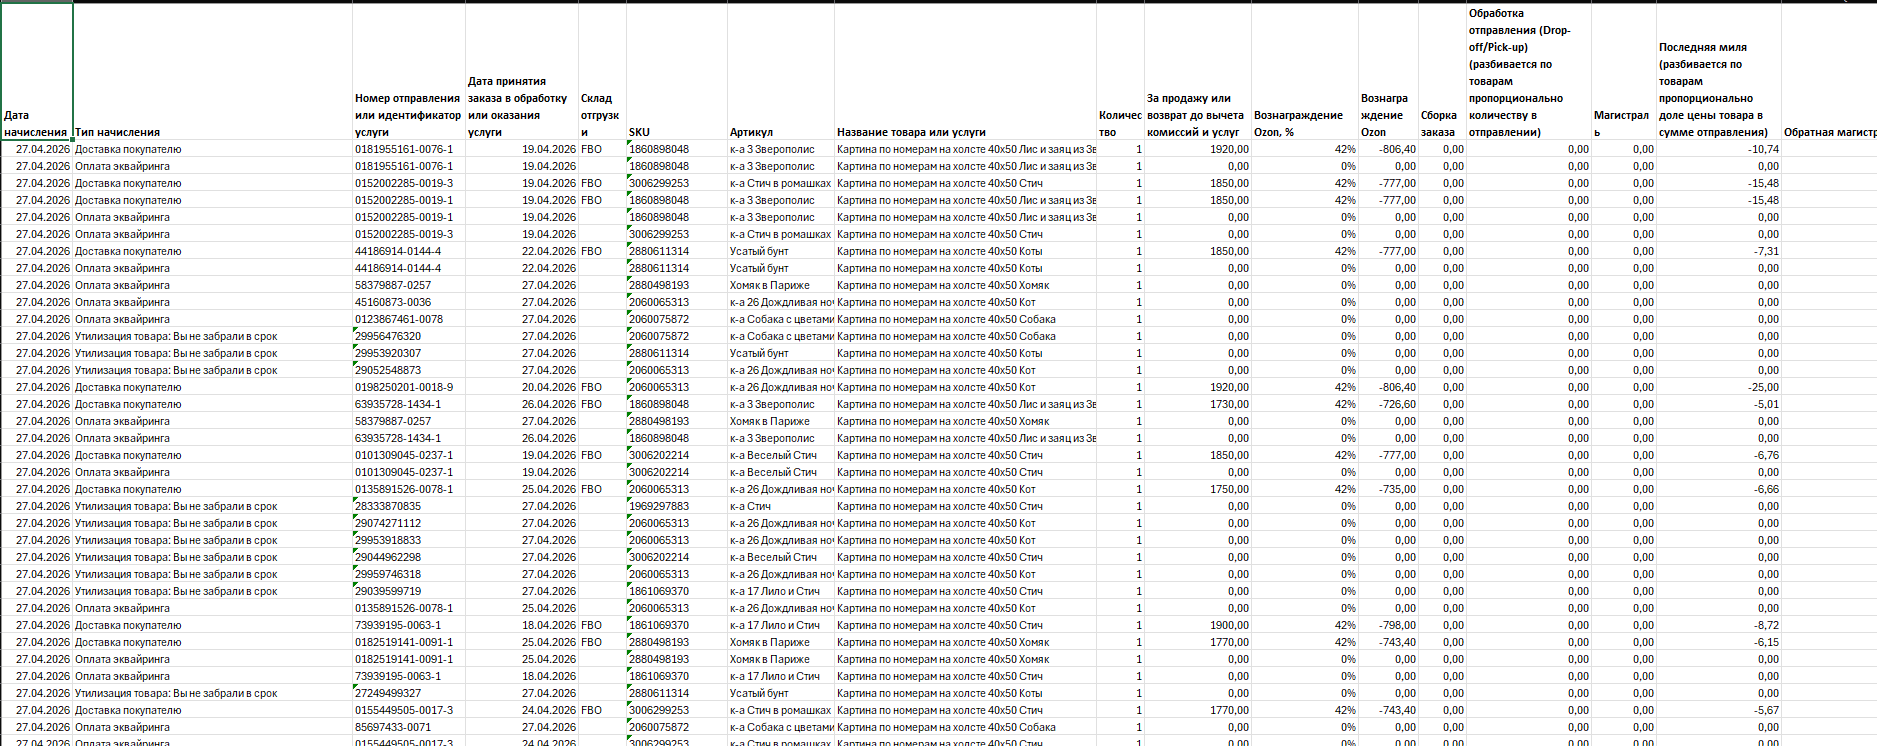
\includegraphics[width=1\textwidth]{../image/screen.png}
    \caption{Пример отчета, выдаваемый маркетплейсом.}
    \label{fig:example01}
\end{figure}

Маркетплейсы дают продавцам два основных варианта доступа к информации: через API платформы и через ручную выгрузку отчетов в форматах csv/xlsx из личного кабинета пользователя. Рассмотрим каждый из них.

\subsection{API отчеты}

API – это набор определенных правил, протоколов и инструментов, которые позволяют одному программному приложению взаимодействовать с другим ~\cite{usingAPI}.
 
С помощью этого инструмента можно получать доступ к данным в реальном моменте времени, управлять приложением по четко сформированным правилам, а также контролировать большие объёмы данных.

Для настройки интеграции по API с маркетплейсами требуется специальный токен, который создается в личном кабинете пользователя.

Из минусов важно упомянуть, что если токеном завладеет злоумышленник, то он получит полный доступ к личному кабинету, сможет изменять любые данные, поэтому возникает вопрос безопасности такой системы~\cite{usingAPI}. 

Помимо этого, у ключей есть срок годности и лимиты запросов, следовательно сами токены нужно обновлять. Так же для создания такой системы потребуется надежная ауте ия пользователя для защиты ключа от посторонних, база данных для хранения информация кабинета и о ключах, а также знания работы с API конкретного маркетплейса, что усложняет разработку~\cite{usingAPI}. 

Но метод получения данных по API является наиболее предпочтительным для разработки веб приложения и автоматизации системы, получаемые данные являются самыми актуальными, которые может предоставить маркетплейс, а их доступность выходит на совершенно новый уровень.

\subsection{Файловые отчеты}
Отчеты о продажах, поступлениях и многом другом предоставляют маркетплейсы, вся информация на момент скачивания отчета является актуальной на сегодняшний день с малейшими погрешностями. Данный подход обладает ключевыми преимуществами, по сравнению с API:

\begin{itemize}
    \item Простота реализации – Такая система не требует обязательной аутентификации пользователя, создания личных токенов и их настройки, использования базы данных для хранения самих токенов, а также сложной логики их обработки. Вся логика сосредоточена на парсинге данных и их последующей обработки для структуризации.
    \item Безопасность – Исключение рисков утечек информации, связанные с хранением и передачей токенов доступа API, так как обработка данных происходит на стороне клиента.
\end{itemize}

\begin{table}[H]
\caption{Сравнение Rest API отчетов и обычных отчетов}
\begin{tabular}{|p{5cm}|p{4cm}|p{4cm}|}
\hline
Критерии & Rest API отчеты & Отчеты \\ \hline
Актуальность данных & Реальное время & На день формирования отчета \\ \hline
Сложность реализации & Высокая & Средняя \\ \hline
Требования безопасности & Высокие & Минимальные \\ \hline
Зависимость от платформы & Высокая & Низкая \\ \hline
Необходимость серверной части & Обязательна & Не обязательна \\ \hline
Автоматизация системы & Наивысшая & Минимальная \\ \hline
\end{tabular}
\end{table}

Для целей данной работы выбран подход с использованием отчётов, получаемых через API токены, так как он позволяет автоматизировать систему, получать самые актуальные данные и контролировать их форматирование. Данный подход обеспечивает необходимый баланс между функциональностью, безопасностью и сложностью реализации.

\section{Использование API}
Решение о выборе архитектурного подхода к интеграции с API является ключевым этапом при создании системы автоматизированного сбора и обработки данных маркетплейса. От правильности этого выбора будет зависеть надежность получения данных, стабильность работы приложения и возможности его дальнейшего масштабирования~\cite{ozonapiAsync}.

В отличие от традиционной веб-разработки, где основное внимание уделяется выбору языка программирования, при работе с API торговых платформ на первый план выходят следующие критерии:

\begin{enumerate}
    \item Протоколы взаимодействия: современные маркетплейсы, используют REST API как основной стандарт обмена данными. REST работает поверх протокола HTTP и использует стандартные методы запросов (GET, POST, PUT, DELETE), что обеспечивает универсальность и простоту интеграции~\cite{ozonapiAsync}.
    \item Форматы обмена данными: API маркетплейсов, используют JSON (JavaScript Object Notation) как основной формат передачи данных. JSON стал отраслевым стандартом благодаря своей легкости, читаемости и совместимости с любыми языками программирования~\cite{ozonapiAsync}.
    \item Аутентификация и безопасность: Работа с API маркетплейсов требует надежной системы аутентификации. Ozon API использует двухкомпонентную систему: Client-ID и API-ключ, которые передаются в заголовках каждого запроса. Это обеспечивает защиту от несанкционированного доступа и позволяет идентифицировать каждое обращение к серверу~\cite{ozonapiAsync}.
    \item Асинхронность операций: Важной особенностью API Ozon является асинхронная модель формирования отчетов. При запросе большого объема данных сервер не возвращает их мгновенно, а создает задачу и предоставляет уникальный идентификатор, по которому впоследствии можно получить готовый отчет. Такой подход позволяет эффективно распределять серверные ресурсы и обрабатывать запросы любого объема~\cite{ozonapiAsync}.
    \item Кроссплатформенность: API-интеграция не привязана к конкретному языку программирования или операционной системе. Любое приложение, способное отправлять HTTP-запросы и обрабатывать JSON-ответы, может взаимодействовать с API Ozon. Это обеспечивает свободу выбора технологий на стороне клиента и возможность поэтапного развития системы~\cite{ozonapiAsync}.
\end{enumerate}

Таким образом, при проектировании системы сбора отчетности выбор делается не столько в пользу конкретного языка программирования, сколько в пользу понимания API маркетплейса, форматов данных и моделей взаимодействия с сервером маркетплейса~\cite{retailcrmOzon}.

\section{Аутентификация и авторизация пользователей в веб-приложениях}

При разработке многопользовательских веб-приложений, работающих с конфиденциальными коммерческими данными, критически важным становится разграничение доступа между пользователями~\cite{authBasics}. Для этого применяются два взаимосвязанных процесса: аутентификация и авторизация. Несмотря на схожесть терминов, они решают разные задачи.

Аутентификация – это процесс проверки подлинности пользователя, то есть подтверждение того, что пользователь является тем, за кого себя выдаёт. В большинстве веб-приложений аутентификация реализуется через ввод пары «логин (email) – пароль»~\cite{authBasics}. Система сравнивает введённые данные с теми, что хранятся в базе данных, и при совпадении предоставляет пользователю доступ~\cite{bookWebAuth}.

Авторизация – это процесс определения прав доступа аутентифицированного пользователя к определённым ресурсам или функциям системы~\cite{authBasics}. Если аутентификация отвечает на вопрос «кто пользователь?», то авторизация – «что пользователь может делать?». В рамках данной работы авторизация реализована на уровне маршрутов: неавторизованный пользователь не может получить доступ к страницам аналитики, даже если введёт их URL вручную~\cite{bookNextjs}.

\subsection{Методы хранения паролей: хеширование и шифрование}

Одной из главных угроз безопасности веб-приложений является хищение и взлом баз данных с учётными записями пользователей~\cite{owaspPasswords}. Хранение паролей в открытом виде недопустимо, так как при утечке базы данных злоумышленник получает полный доступ к аккаунтам всех пользователей. Для защиты паролей применяются два основных подхода: шифрование и хеширование~\cite{bookCryptography}.

Шифрование – это двусторонний процесс преобразования данных с использованием ключа. Зашифрованные данные можно расшифровать обратно в исходный текст при наличии правильного ключа. Шифрование применяется для передачи данных по сети (например, HTTPS/TLS) или для хранения данных, которые могут понадобиться в исходном виде. Однако для хранения паролей шифрование не подходит, так как злоумышленник, получивший доступ к базе данных и ключу шифрования, сможет расшифровать все пароли.

Хеширование – это одностороннее преобразование данных в строку фиксированной длины (хеш, или хеш-сумму). Главное свойство хеширования – необратимость: по полученному хешу невозможно восстановить исходный пароль~\cite{bcryptDocs}. При регистрации пользователя система вычисляет хеш пароля и сохраняет именно его. При последующем входе система повторно вычисляет хеш от введённого пароля и сравнивает его с сохранённым хешем. Если хеши совпадают – пароль введён верно. Сам исходный пароль при этом нигде не хранится.

Однако простые хеш-функции уязвимы для атак по словарям и радужным таблицам. Злоумышленник может предварительно вычислить хеши для всех распространённых паролей и быстро найти соответствие. Для защиты от таких атак применяются два механизма: соль и адаптивное хеширование~\cite{bcryptDocs}.

Модификатор входа хеш-функции – это случайная строка, которая добавляется к паролю перед хешированием. Соль генерируется индивидуально для каждого пользователя и сохраняется вместе с хешем~\cite{owaspPasswords}. Даже если два пользователя имеют одинаковый пароль, благодаря разным солям их хеши будут различаться. Это делает атаки по радужным таблицам неэффективными.

Адаптивное хеширование – это метод, при котором функция хеширования выполняется многократно (обычно тысячи или десятки тысяч раз), что значительно увеличивает время вычисления хеша. Для пользователя это замедление незаметно (доли секунды), но для злоумышленника, перебирающего миллионы паролей, такое замедление делает атаку практически невозможной. В данной работе используется библиотека bcrypt, которая реализует адаптивное хеширование с автоматическим добавлением модификатора входа хеш-функции~\cite{bcryptDocs}.

\subsection{Управление сессиями: JWT и HTTP-only cookies}

После успешной аутентификации приложению необходимо запомнить, что пользователь вошёл в систему, чтобы не требовать повторного ввода пароля при каждом переходе между страницами. Для этого используются механизмы управления сессиями~\cite{jwtIntro}. В современных веб-приложениях наиболее распространены два подхода: серверные сессии (с хранением состояния на сервере) и токен-ориентированная аутентификация (клиентские токены). В данной работе реализован второй подход с использованием JWT~\cite{bookJWT}.

JWT (JSON Web Token) – это открытый стандарт (RFC 7519) для создания компактных и самодостаточных токенов, передающих информацию между сторонами в виде JSON-объекта~\cite{jwtIntro}. JWT состоит из трёх частей, разделённых точками:
\begin{itemize}
    \item Header (заголовок) – содержит информацию о типе токена и алгоритме подписи (например, HS256);
    \item Payload (полезная нагрузка) – содержит утверждения о пользователе: идентификатор, email, время создания и время истечения токена;
    \item Signature (подпись) – создаётся путём шифрования заголовка и полезной нагрузки с использованием секретного ключа. Подпись гарантирует, что токен не был изменён после создания~\cite{jwtIntro}.
\end{itemize}

Преимущества JWT:

\begin{enumerate}
    \item Самодостаточность – токен содержит всю необходимую информацию о пользователе, что снижает нагрузку на сервер~\cite{jwtIntro};
    \item Масштабируемость – серверу не нужно хранить состояние сессии, что упрощает горизонтальное масштабирование~\cite{bookJWT};
    \item Механизм истечения – токены автоматически становятся недействительными по истечении заданного времени~\cite{jwtIntro}.
\end{enumerate}

Однако JWT-токен необходимо безопасно хранить на клиенте. Наиболее распространённый способ – использование HTTP-only cookies~\cite{cookieSecurity}.

HTTP-only cookies – это файлы cookie, которые имеют флаг HttpOnly. Этот флаг запрещает доступ к cookie из клиентского JavaScript-кода, что эффективно защищает токен от XSS-атак (межсайтовый скриптинг)~\cite{owaspXSS}. Даже если злоумышленник внедрит вредоносный скрипт на страницу, он не сможет украсть JWT-токен. Дополнительно устанавливаются флаги Secure (передача только по HTTPS) и SameSite=lax (защита от CSRF-атак)~\cite{cookieSecurity}. В разработанном приложении при успешном входе сервер устанавливает HTTP-only cookie с JWT-токеном, и при каждом последующем запросе браузер автоматически отправляет эту cookie на сервер.

\subsection{Защита маршрутов: proxy (middleware)}

Для предотвращения доступа неавторизованных пользователей к защищённым разделам веб-приложения необходимо проверять наличие валидной сессии при каждом переходе между страницами. В Next.js эта задача решается с помощью механизма middleware (в версии 16 переименован в proxy)~\cite{nextjsMiddleware}.

Proxy-функция выполняется на сервере перед обработкой каждого входящего запроса. Она проверяет наличие и валидность JWT-токена в cookie и принимает решение:

\begin{itemize}
    \item Если пользователь не авторизован и пытается зайти на защищённую страницу (аналитика, дашборд) – происходит перенаправление на страницу входа~\cite{nextjsMiddleware};
    \item Если пользователь авторизован и пытается зайти на страницу входа или регистрации – происходит перенаправление на главную страницу~\cite{nextjsMiddleware}.
\end{itemize}

Такой подход обеспечивает единую точку контроля доступа и исключает необходимость дублировать проверки на каждой странице~\cite{bookNextjs}.



\section{Хранение учётных записей}

Для постоянного хранения зарегистрированных пользователей в веб-приложении используется база данных SQLite. Это легковесная встраиваемая система управления базами данных, которая не требует отдельного серверного процесса и хранит все данные в одном файле (users.db). Таблица пользователей содержит следующие поля:

\begin{itemize}
\item id – уникальный идентификатор пользователя (формат UUID);
\item email – адрес электронной почты (используется в качестве логина);
\item password\_hash – хеш пароля, сгенерированный bcrypt;
\item created\_at – дата и время регистрации.
\end{itemize}

Выбор SQLite обусловлен простотой развёртывания, отсутствием необходимости в настройке отдельного сервера баз данных и достаточной производительностью для малого и среднего количества пользователей и данных.

\section{Используемые технологии в проекте}
В разработанном веб-приложении для реализации аутентификации и авторизации применяются следующие технологии:

\begin{table}[H]
\caption{Технологии и компоненты системы аутентификации}
\begin{tabular}{|l|l|l|}
\hline
Компонент & Технология & Назначение \\ \hline
Хеширование паролей & bcrypt & Адаптивное хеширование \\ \hline
Токены сессий & JWT & Создание токенов \\ \hline
Хранение токенов & HTTP-only cookies & Хранение токенов, защита от XSS \\ \hline
Защита маршрутов & Next.js proxy & Проверка авторизации \\ \hline
База данных & SQLite & Хранение учётных записей \\ \hline
Язык реализации & TypeScript & Типизированная надстройка \\ \hline
\end{tabular}
\end{table}

Таким образом, выбранный комплекс технологий обеспечивает надёжную защиту пользовательских данных, удобство использования и масштабируемость системы.

\begin{table}[H]
\caption{Технические инструменты разработки сайта}
\begin{tabular}{|l|l|}
\hline
Назначение & Технология \\ \hline
Разметка страниц & HTML5 \\ \hline
Стилизация и адаптивность & CSS + Tailwind CSS \\ \hline
Язык программирования & TypeScript \\ \hline
Фреймворк & Next.js 16 (App Router) \\ \hline
API-запросы & Fetch API / HTTPS \\ \hline
Авторизация & JWT + bcrypt + HTTP-only cookies \\ \hline
База данных пользователей & SQLite \\ \hline
Работа с Excel/CSV & XLSX \\ \hline
Защита маршрутов & Proxy Next.js \\ \hline
\end{tabular}
\end{table}

 %главы
\chapter{ПРОЕКТИРОВАНИЕ И РЕАЛИЗАЦИЯ АРХИТЕКТУРЫ ВЕБ-ПРИЛОЖЕНИЯ}

\section{Анализ структуры исходных данных}
Для корректной обработки информации маркетплейсов исследованы форматы и структура ключевых отчётов, получаемых с помощью API: отчёт о продажах (CSV) и отчёт об остатках по кластерам (XLSX). Данные форматы являются стандартизированными и машинно-читаемыми, что позволяет автоматизировать их обработку.

\subsection{Отчет о продажах (CSV)}
Отчёт содержит транзакционные данные, где каждая строка соответствует товарной позиции в заказе. Названия столбцов для анализа отчета: 

\begin{enumerate}
\item Принят в обработку – дата оформления заказа;
\item Статус – статус заказа («Доставлен»/«Отменен»/«Доставляется»);
\item Сумма отправления – стоимость заказа;
\item Название товара – наименование товара на маркетплейсе;
\item Количество – количество товаров в одном заказе.
\end{enumerate}

\subsection{Отчёт об остатках по кластерам (XLSX)}
Отчёт отражает распределение товарных запасов по складам (кластерам) маркетплейса. Ключевые поля:

\begin{enumerate}
\item Название товара – наименование товара на маркетплейсе;
\item Кластер – Город размещения склада;
\item Ликвидность – на сколько интересным товар в кластере;
\item Среднесуточные продажи – среднее арифметическое всех продаж;
\item Остатки на складах – количество остатков товара в кластере.
\end{enumerate}

Помимо вышесказанного, требуется произвести нормализацию данных для обеспечения устойчивости к изменениям формата отчетов. Алгоритм реализован по методу адаптивного парсинга, который идентифицирует колонки по их содержанию (например, поиск подстроки «Количество»). 

Таким образом, структура исходных отчётов содержит все необходимые данные для реализации трёх модулей аналитики: расчёта юнит-экономики, анализа динамики продаж и прогнозирования остатков на кластерах.

\section{Адаптивный парсинг и валидация данных}

Исходные отчёты маркетплейсов (CSV и XLSX) не имеют жёстко фиксированной структуры: маркетплейсы могут изменять порядок столбцов, добавлять новые поля или переименовывать существующие. Прямая привязка к индексам столбцов привела бы к частым ошибкам при обновлении форматов выгрузки. Для решения этой проблемы реализован адаптивный парсинг – метод, при котором система автоматически идентифицирует необходимые столбцы, по ключевым словам, в заголовках, независимо от их позиции в файле.

\subsection{Адаптивный парсинг веб – сайта}

На рисунке 2.1 представлена блок-схема алгоритма адаптивного парсинга применительно к отчёту о продажах. Алгоритм выполняет следующие действия:

\begin{enumerate}
\item Проверка файла – если файл пуст или не содержит заголовков, обработка прерывается с сообщением об ошибке;
\item Парсинг заголовков – считываются названия всех столбцов;
\item Поиск целевых колонок – для каждого аналитического поля (дата, название товара, количество, статус, сумма) выполняется поиск подстроки в заголовках. Поиск регистронезависимый названий, допускаются варианты количество, кол-во, quantity;
\item Фиксация индексов – найденные индексы столбцов запоминаются;
\item Заполнение данных – построчный обход файла, извлечение значений по зафиксированным индексам и преобразование типов (даты, числа);
\end{enumerate}

Если какой-либо обязательный столбец не найден, алгоритм возвращает ошибку с указанием отсутствующего поля. Алгоритм парсинга показан на рисунке 2.1.

\begin{figure}[h]
    \centering
    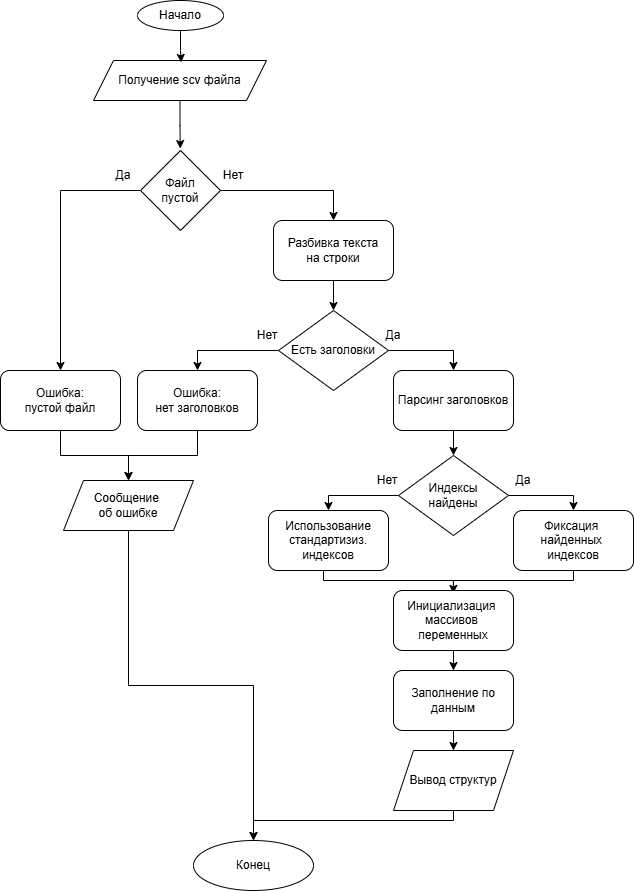
\includegraphics[width=0.9\textwidth]{../image/screen2.png}
    \caption{Пример парсинга файла и валидации данных.}
    \label{fig:example01}
\end{figure}

\subsection{Валидация и обработка ошибок}
После извлечения данных выполняется валидация:
\begin{itemize}
\item проверка формата дат;
\item приведение числовых полей к типу number;
\item фильтрация строк по статусу заказа (только доставленные заказы участвуют в аналитике);
\item отбрасывание строк с некорректными или пустыми значениями.
\end{itemize}

Для XLSX-файлов (отчёт об остатках) алгоритм дополняется выбором активного листа и поиском специфических полей: Кластер, Ликвидность, Среднесуточные продажи, Остатки на складах, Дней без остатка.

При возникновении любой ошибки пользователь получает информативное сообщение на русском языке с указанием причины. Это позволяет быстро исправить проблему без анализа технических логов.

\section{Кластерный анализ }

На основе отчёта об остатках по кластерам (XLSX) разработан модуль кластерного анализа, который позволяет оценить распределение товарных запасов по складам маркетплейса, выявить неликвидные остатки и сформировать рекомендации по пополнению.

\subsection{Исходные данные для анализа}

Модуль использует следующие поля отчёта (см. рис. 2.2.):

\begin{itemize}
\item Товар – id, наименование/артикул товара;
\item Кластер – id, город/название кластера;
\item Остаток товара в кластере – id, товар\_id, кластер\_id, остаток, среднесуточные продажи за 28 дней, ликвидность, дата выгрузки;
\item Прогноз по товару – товар\_id, суммарный остаток, суммарные продажи, дней до исчерпания, рекомендация;
\item Прогноз по кластеру – id, товар\_id, кластер\_id, дней до исчерпания, рекомендация, цветовая зона.
\end{itemize}

Связи между сущностями:

\begin{enumerate}
\item Товар (1) – (М) Остаток товара в кластере. Один товар может храниться во многих кластерах (складах);
\item Кластер (1) – (М) Остаток товара в кластере. В одном кластере может храниться много товаров;
\item Остаток товара в кластере (1) – (1) Прогноз по кластеру. Каждая запись остатка порождает один прогноз для конкретного кластера;
\item Товар (1) – (1) Прогноз по товару. Каждый товар имеет один итоговый прогноз (агрегированный по всем кластерам).
\end{enumerate}



\begin{figure}[h]
    \centering
    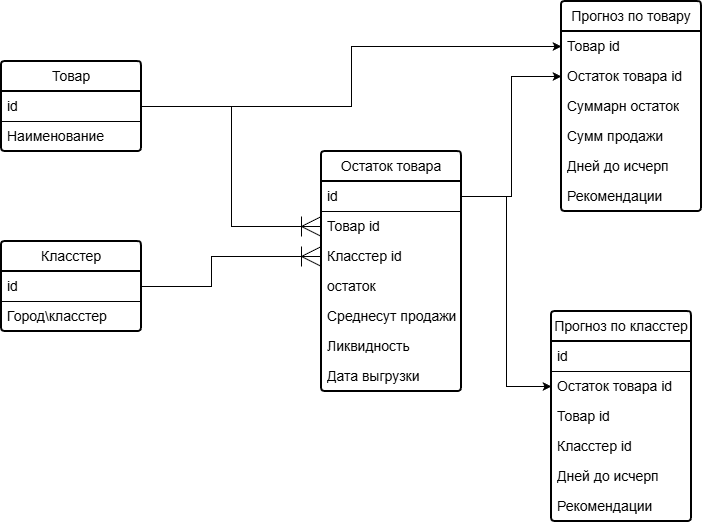
\includegraphics[width=1\textwidth]{../image/er диаграмма класстерного анализа.drawio.png}
    \caption{ER-диаграмма взаимосвязей.}
    \label{fig:example01}
\end{figure}

\subsection{Алгоритм кластерного анализа}

Вычисления выполняются в следующем порядке:

\begin{enumerate}
\item Расчёт уровня локализации товара:

Уровень локализации показывает, в скольких кластерах из всех возможных товар уже представлен:

\begin{equation}
\text{Уровень локализации} = \frac{\text{Количество кластеров с остатком} > 0}{\text{Общее количество кластеров}} \times 100\%
\end{equation}

Чем выше уровень, тем шире географическое присутствие товара. Низкий уровень ($<30\%$) указывает на потенциал расширения.

\item Прогноз остатков (дней до исчерпания):

Для каждого кластера, где товар присутствует, вычисляется, на сколько дней хватит текущего запаса при текущих среднесуточных продажах:

\begin{equation}
\text{Дней до исчерпания} = \frac{\text{Остаток на складе}}{\text{Среднесуточные продажи}}
\end{equation}

Если знаменатель равен нулю (продаж нет), прогноз считается бесконечным – товар не продаётся.

\item Классификация зон пополнения:

На основе прогноза кластеры разделяются на три зоны:

\begin{itemize}
\item красная зона (дней $<30$) – требуется срочное пополнение;
\item жёлтая зона ($30$–$60$ дней) – плановое пополнение в ближайшее время;
\item зелёная зона ($>60$ дней) – пополнение не требуется.
\end{itemize}

\item Оценка ликвидности:

Ликвидность определяется на основе переданного показателя из отчёта, и классифицируются по формуле (2.3):

\begin{equation}
\text{Ликвидность} = 
\begin{cases}
\text{Высокая}, & \text{среднесуточные продажи} > 50; \\[4pt]
\text{Средняя}, & \text{если } 10 \leq \text{продажи} \leq 50; \\[4pt]
\text{Низкая}, & \text{если продажи} < 10.
\end{cases}
\end{equation}

Товары с низкой ликвидностью и большими остатками маркируются как «замороженный запас» – рекомендуется уценка или перемещение в более востребованные кластеры.

\item Формирование рекомендаций:

На выходе модуль формирует:

\begin{itemize}
\item Сводную таблицу по каждому товару: кластеры, остатки, прогноз дней, зона пополнения;
\item Список кластеров, требующих срочной поставки;
\item Перечень неликвидных остатков с предложениями по оптимизации.
\end{itemize}

\end{enumerate}

\subsection{Практическая ценность}

Разработанный алгоритм позволяет продавцу автоматически получать ответы на ключевые вопросы:

\begin{itemize}
\item В какие кластеры нужно поставить товар и в каком объёме;
\item В каких кластерах слабая оборачиваемость;
\item Насколько равномерно товар распределён по регионам.
\end{itemize}

Это сокращает время на анализ остатков с нескольких часов до нескольких минут и минимизирует риск упущенных продаж из-за отсутствия товара в востребованных кластерах.

\section{Реализация API}

\subsection{Общая методология работы с API}

Работа с любым современным REST API, например Ozon Seller API, строится на нескольких фундаментальных принципах, которые необходимо учитывать при разработке приложений [8].

Архитектура клиент-серверного взаимодействия, для примера возьмем OZON API, организовано по классической модели запрос-ответ. Клиентское приложение инициирует соединение, отправляя HTTP-запросы на серверы Ozon. Сервер обрабатывает запрос и возвращает ответ в формате JSON. Все запросы выполняются по защищенному протоколу HTTPS, что гарантирует шифрование передаваемых данных и защиту от перехвата конфиденциальной информации.

Ключевым требованием для работы с API является наличие действующих учетных данных продавца. Для работы потребуется client id и API токен, при каждом запросе к API эти данные передаются в HTTP-заголовках, что обеспечивает идентификацию отправителя и проверку его прав доступа.

Особенностью работы с отчетами в Ozon API является асинхронная модель обработки запросов. При запросе большого объема данных сервер не возвращает их мгновенно, а создает задачу на формирование отчета и предоставляет уникальный идентификатор (code), по которому впоследствии можно получить готовый отчет. Такой подход позволяет эффективно распределять серверные ресурсы и обрабатывать запросы любого объема без риска превышения таймаутов соединения.

Для получения отчетов по API требуется использования трех ключевых методов Ozon Seller API, которые в совокупности реализуют полный цикл получения отчетов по отправлениям [8].

\subsection{Метод создания отчета: POST /v1/report/postings/create}

Данный метод инициирует процесс формирования отчета по отправлениям за указанный временной период [8].

В теле запроса клиент передает фильтр с параметрами выборки:

\begin{code}
\captionof{listing}{Фильтры с параметрами выборки для интеграции API Ozon seller c веб приложением}
\label{code:openmp}
\vspace{-0.75cm}\begin{minted}[mathescape,linenos,frame=lines,breaklines]{C}
const requestBody = {
    filter: {
        processed_at_from: formatDate(fromDate),
        processed_at_to: formatDate(toDate),
        delivery_schema: [deliverySchema],
        statuses: []
    },
    language: 'DEFAULT'
};
\end{minted}
\end{code}

Критически важным требованием спецификации является передача параметра delivery schema в виде массива, даже если указывается только одно значение (например, ["fbo"] или ["fbs"]). В случае успешного создания задачи сервер возвращает объект с уникальным кодом отчета. Этот код сохраняется в приложении и используется для последующей проверки статуса готовности [8].

\subsection{Метод проверки статуса: POST /v1/report/info}

Поскольку формирование отчета может занимать от нескольких секунд до нескольких минут (в зависимости от объема данных и загрузки серверов), необходим механизм проверки готовности результата. Метод info принимает код отчета и возвращает актуальную информацию о его состоянии [8].

\begin{code}
\captionof{listing}{Реализация цикла опроса сервера для получения отчета с экспоненциальной задержкой}
\label{code:openmp}
\vspace{-0.75cm}\begin{minted}[mathescape,linenos,frame=lines,breaklines]{C}
for (let i = 0; i < 30; i++) {
    const response = await fetch('https://api-seller.ozon.ru/v1/report/info', {
        method: 'POST',
        headers: { ... },
        body: JSON.stringify({ code })
    });

    const data = await response.json();
    if (data.result.status === 'success') {
        return data.result;
    }
    await sleep(2000);
}
\end{minted}
\end{code}

В процессе работы метод может возвращать следующие статусы [8]:

\begin{itemize}
\item pending / waiting / processing — отчет еще формируется, необходимо повторить запрос позже;
\item success — отчет готов к скачиванию, в ответе присутствует прямая ссылка на файл;
\item error — при формировании отчета произошла ошибка (например, указан некорректный период).
\end{itemize}

При успешной готовности метод возвращает объект, содержащий ссылку для скачивания сформированного файла.

\subsection{Получение отчета }

Заключительный этап — получение файла отчета по предоставленной ссылке. В отличие от предыдущих методов, этот запрос не требует специальных заголовков авторизации, так как ссылка является временной и одноразовой.

В процессе разработки было установлено, что файлы отчетов могут передаваться в различных форматах (CSV, XLSX) и кодировках. Наиболее надежный подход — сохранять файл в бинарном виде, полностью сохраняя исходное форматирование:

\begin{code}
\captionof{listing}{Реализация цикла опроса сервера для получения отчета с экспоненциальной задержкой}
\label{code:openmp}
\vspace{-0.75cm}\begin{minted}[mathescape,linenos,frame=lines,breaklines]{C}
const response = await fetch(fileUrl, {
    agent: new https.Agent({ keepAlive: true })
});

const buffer = await response.buffer();
fs.writeFileSync(filePath, buffer);

\end{minted}
\end{code}

В некоторых случаях Ozon возвращает файлы в кодировке Windows-1251, что при открытии в современных редакторах приводит к отображению нечитаемых символов. Для решения этой проблемы в приложении реализована автоматическая конвертация.

\begin{code}
\captionof{listing}{Реализация цикла опроса сервера для получения отчета с экспоненциальной задержкой}
\label{code:openmp}
\vspace{-0.75cm}\begin{minted}[mathescape,linenos,frame=lines,breaklines]{C}
try {
    content = buffer.toString('utf8');
} catch {
    content = iconv.decode(buffer, 'win1251');
}
\end{minted}
\end{code}

\section{Модульная структура веб API системы}

Приложение построено по модульному принципу, где каждая функция отвечает за отдельный этап взаимодействия с API [8]:

\begin{table}[H]
\caption{Функции для работы с отчетами Ozon API}
\label{tab:report-functions}
\begin{tabular}{|l|l|l|l|}
\hline
Функция & Назначения & Входные параметры & Возвращаемое значение \\ \hline
createReport & Создание отчета & Параметры фильтрации & Код отчета \\ \hline
waitForReport & Проверка статуса & Код отчета & Информация с ссылкой \\ \hline
downloadReport & Скачивание файла & URL, тип отчета & Путь к сохраненному файлу \\ \hline
\end{tabular}
\end{table}

\section{Обработка ошибок и исключений}
Все запросы к API обернуты в блоки try/catch для корректной обработки возможных сбоев:

\begin{itemize}
\item Ошибки сети — таймауты, разрывы соединения;
\item Ошибки авторизации — неверный Client ID или API-ключ;
\item Ошибки валидации — некорректные параметры запроса;
\item Ошибки сервера — временные проблемы на стороне Ozon.
\end{itemize}

\begin{code}
\captionof{listing}{Обработка сбоев}
\label{code:openmp}
\vspace{-0.75cm}\begin{minted}[mathescape,linenos,frame=lines,breaklines]{C}
try {
    const response = await fetch(url, options);
    const data = await response.json();
    
    if (!response.ok) {
        throw new Error(`Ошибка API: ${JSON.stringify(data)}`);
    }
    
    return data.result;
} catch (error) {
    log(` Ошибка: ${error.message}`, 'ERROR');
    throw error;
}

\end{minted}
\end{code}

\section{Анализ структуры входных данных}
Для корректной обработки информации маркетплейсов исследованы форматы и структура ключевых отчётов: отчёт о продажах (CSV) и отчёт об остатках по кластерам (XLSX). Данные форматы являются стандартизированными и машинно-читаемыми, что позволяет автоматизировать их обработку.

\subsection{Отчет о продажах (CSV) }

Отчёт содержит транзакционные данные, где каждая строка соответствует товарной позиции в заказе. Названия столбцов для анализа отчета:

\begin{enumerate}
\item Принят в обработку – дата оформления заказа;
\item Статус – статус заказа («Доставлен»/«Отменен»/«Доставляется»);
\item Сумма отправления – стоимость заказа;
\item Название товара – наименование товара на маркетплейсе;
\item Количество – количество товаров в одном заказе.
\end{enumerate}

\subsection{Отчёт об остатках по кластерам (XLSX)}

Отчёт отражает распределение товарных запасов по складам (кластерам) маркетплейса. Ключевые поля:

\begin{enumerate}
\item Название товара – наименование товара на маркетплейсе;
\item Кластер – Город размещения склада;
\item Ликвидность – на сколько интересным товар в кластере;
\item Среднесуточные продажи – среднее арифметическое всех продаж;
\item Остатки на складах – количество остатков товара в кластере.
\end{enumerate}

Помимо вышесказанного, требуется произвести нормализацию данных для обеспечения устойчивости к изменениям формата отчетов. Алгоритм реализован по методу адаптивного парсинга, который идентифицирует колонки по их содержанию (например, поиск подстроки «Количество»).

Таким образом, структура исходных отчётов содержит все необходимые данные для реализации трёх модулей аналитики: расчёта юнит-экономики, анализа динамики продаж и прогнозирования остатков на кластерах.

\section{Проектирование системы обработки данных}
Архитектура системы построена на принципах клиент-серверной модели с обработкой на стороне клиента. Основная цель архитектуры – преобразование сырых данных из форматов CSV/XLSX в структурированные аналитические показатели через последовательные обработки.

Блок-схема процесса обработки данных представлена на рисунке 2.1

\begin{figure}[h]
    \centering
    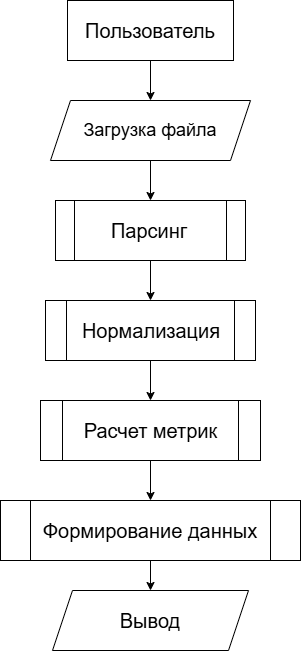
\includegraphics[width=0.2\textwidth]{../image/screen3.png}
    \caption{Архитектура обработки данных.}
    \label{fig:example02}
\end{figure}

\subsection{Алгоритм парсинга и нормализации данных}

Алгоритм парсинга получаемых API CSV-отчетов (данные о продажах) предназначен для преобразования текстовых CSV-файлов в структурированные данные. Процесс состоит из следующих шагов:

\begin{enumerate}
\item Получение разрешения на доступ к API отчетам;
\item Запрос на получение API отчета;
\item Получение API отчета;
\item Чтение файла – получение CSV как текстовой строки;
\item Разделение на строки – разбиение текста по символам новой строки;
\item Определение структуры:
\begin{itemize}
\item Первая строка обрабатывается как заголовок;
\item Определяются индексы нужных колонок по их названиям;
\item Если колонка не найдена по названию, используется стандартный индекс.
\end{itemize}
\item Обработка данных – для каждой строки:
\begin{itemize}
\item Извлечение значений по определенным индексам;
\item Парсинг дат с учетом разных форматов;
\item Классификация заказов по статусам.
\end{itemize}
\end{enumerate}

Алгоритм парсинга XLSX-отчетов (данные об остатках по кластерам) предназначен для обработки Excel-файлов с информацией о распределении товаров по складам:

\begin{enumerate}
\item Чтение файла – получение XLSX файла;
\item Поиск нужного листа – идентификация рабочего листа с данными;
\item Определение начала данных – пропуск заголовочных строк (первые 4 строки);
\item Извлечение данных – чтение значений из конкретных колонок:
\begin{itemize}
\item Колонка F – название кластера (склада);
\item Колонка B – название товара;
\item Колонка K – количество остатков;
\item Колонка L – товары в процессе подготовки;
\item Колонка O – товары с истекающим сроком;
\item Колонка V – возвращаемые товары.
\end{itemize}
\item Фильтрация – удаление служебных и пустых строк;
\item Структурирование – преобразование в табличную форму (товары + кластеры);
\end{enumerate}

\subsection{Алгоритм валидации данных}

Процесс проверки корректности вводимых и обрабатываемых данных:

\begin{enumerate}
\item Проверка типов данных – соответствие ожидаемым типам;
\item Валидация числовых значений:
\begin{itemize}
\item Проверка на числовой тип;
\item Проверка на отрицательные значения;
\item Обработка некорректных значений (замена на 0).
\end{itemize}
\item Проверка форматов:
\begin{itemize}
\item Валидация форматов дат;
\item Проверка текстовых полей на наличие данных.
\end{itemize}
\item Визуальная индикация – выделение полей с ошибками;
\end{enumerate}

Данная архитектура обеспечивает надежную обработку данных без необходимости в серверной инфраструктуре, что соответствует требованиям доступности и безопасности системы.

\section{Авторизация пользователей}

Для разграничения доступа к аналитическим данным в веб-приложении реализована подсистема аутентификации и авторизации. Она обеспечивает регистрацию новых пользователей, вход зарегистрированных пользователей, защиту маршрутов от несанкционированного доступа и безопасное хранение учётных данных. Система построена на следующих компонентах.

\subsection{Регистрация и вход пользователей}

Регистрация нового пользователя выполняется по паре «email – пароль». При регистрации пользователь указывает свой email и пароль (минимальная длина — 6 символов). Сервер проверяет уникальность email — если пользователь с таким адресом уже существует, возвращается ошибка. Пароль никогда не хранится в открытом виде, а подвергается хешированию с помощью библиотеки bcrypt. При входе пользователь вводит email и пароль, сервер находит запись в базе данных, сравнивает хеш введённого пароля с сохранённым и при совпадении открывает доступ.

\begin{code}
\captionof{listing}{Хеширование пароля при регистрации}
\label{code:openmp}
\vspace{-0.75cm}\begin{minted}[mathescape,linenos,frame=lines,breaklines]{C}
const salt = await bcrypt.genSalt(10);
const passwordHash = await bcrypt.hash(password, salt);
\end{minted}
\end{code}

\begin{code}
\captionof{listing}{Сравнение пароля при входе}
\label{code:openmp}
\vspace{-0.75cm}\begin{minted}[mathescape,linenos,frame=lines,breaklines]{C}
const isValid = await bcrypt.compare(password, user.password_hash);
\end{minted}
\end{code}

\subsection{Управление сессией с помощью JWT-токенов}

После успешной аутентификации сервер генерирует JWT-токен (JSON Web Token), который содержит идентификатор пользователя и его email. Токен подписывается секретным ключом, хранящимся в переменных окружения, и имеет ограниченное время жизни (7 дней). Это позволяет автоматически завершать сессию по истечении срока без необходимости хранить состояние на сервере.

\begin{code}
\captionof{listing}{Создание JWT-токена}
\label{code:openmp}
\vspace{-0.75cm}\begin{minted}[mathescape,linenos,frame=lines,breaklines]{C}
const payload = { userId: user.id, email: user.email };
const token = jwt.sign(payload, process.env.JWT_SECRET, { expiresIn: '7d' });
\end{minted}
\end{code}

\subsection{Безопасное хранение токена}

Сгенерированный JWT-токен устанавливается в HTTP-only cookie. Флаг httpOnly запрещает доступ к cookie из клиентского JavaScript-кода, что эффективно защищает токен от XSS-атак. Дополнительно устанавливаются флаги sameSite=lax (защита от CSRF) и secure в production-среде (передача только по HTTPS). При каждом последующем запросе браузер автоматически отправляет эту cookie на сервер.



\begin{code}
\captionof{listing}{Установка HTTP-only cookie}
\label{code:openmp}
\vspace{-0.75cm}\begin{minted}[mathescape,linenos,frame=lines,breaklines]{C}
response.cookies.set({
  name: 'session',
  value: token,
  httpOnly: true,
  path: '/',
  maxAge: 60 * 60 * 24 * 7,
  sameSite: 'lax',
});
\end{minted}
\end{code}

\subsection{Защита маршрутов (middleware/proxy)}
Для предотвращения доступа неавторизованных пользователей к защищённым разделам приложения (страницы аналитики, дашборд) реализован middleware-компонент (в Next.js версии 16 называется proxy.ts). Функция выполняется на сервере перед обработкой каждого входящего запроса, проверяет наличие и валидность JWT-токена в cookie и принимает решение:

Если пользователь не авторизован и пытается зайти на защищённую страницу – происходит перенаправление на страницу входа (/login);

Если пользователь авторизован и пытается зайти на страницу входа или регистрации – перенаправление на главную страницу (/);

Если пользователь авторизован и запрашивает разрешённую страницу – запрос пропускается.



\begin{code}
\captionof{listing}{Пример middleware-проверки}
\label{code:openmp}
\vspace{-0.75cm}\begin{minted}[mathescape,linenos,frame=lines,breaklines]{C}
const token = request.cookies.get('session')?.value;
const isAuthenticated = token ? verifySessionToken(token) !== null : false;

if (!isAuthenticated && !isPublicPath) {
  return NextResponse.redirect(new URL('/login', request.url));
}
\end{minted}
\end{code}

\subsection{База данных пользователей}
Для постоянного хранения учётных записей используется реляционная база данных. Таблица users содержит следующие поля:

\begin{table}[H]
\caption{Структура таблицы пользователей}
\label{tab:users}
\begin{tabular}{|l|l|l|}
\hline
\textbf{Поле} & \textbf{Тип} & \textbf{Описание} \\ \hline
id & TEXT (PRIMARY KEY) & Уникальный идентификатор пользователя (UUID) \\ \hline
email & TEXT (UNIQUE) & Адрес электронной почты (используется как логин) \\ \hline
password\_hash & TEXT & Хеш пароля, сгенерированный bcrypt \\ \hline
created\_at & DATETIME & Дата и время регистрации \\ \hline
\end{tabular}
\end{table}

\subsection{Выход из системы}
При нажатии кнопки «Выйти» клиент отправляет запрос на сервер, который удаляет cookie с токеном сессии. После этого пользователь перенаправляется на страницу входа.

\begin{code}
\captionof{listing}{Выход из системы}
\label{code:openmp}
\vspace{-0.75cm}\begin{minted}[mathescape,linenos,frame=lines,breaklines]{C}
response.cookies.delete('session');
return NextResponse.redirect(new URL('/login', request.url));
\end{minted}
\end{code}

\subsection{Схема работы авторизации}

На рисунке 2.4 представлена общая схема работы подсистемы авторизации:

Пользователь регистрируется → пароль хешируется → сохраняется в БД;

Пользователь входит → сервер проверяет пароль → генерирует JWT → устанавливает HTTP-only cookie;

При переходе на любую страницу middleware проверяет валидность cookie;

При выходе cookie удаляется.

Таким образом, реализованная подсистема обеспечивает надёжную защиту пользовательских данных, удобство использования и масштабируемость. Все пароли хранятся в хешированном виде, токены сессий защищены от XSS-атак, а маршруты централизованно контролируются через middleware.

\begin{figure}[pt]
    \centering
    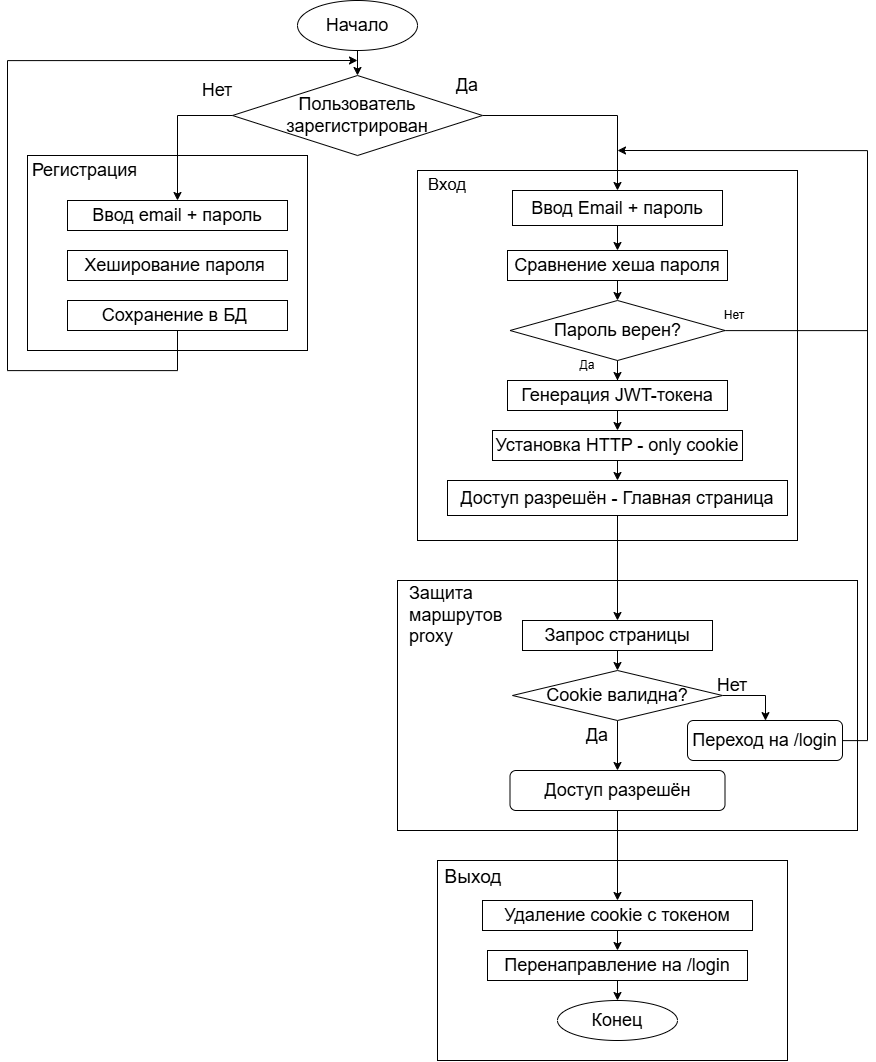
\includegraphics[width=0.7\textwidth]{../image/screen4.png}
    \caption{Схема работы системы авторизации.}
    \label{fig:example02}
\end{figure}
\chapter{ТЕСТИРОВАНИЕ РАЗРАБОТАННОГО ВЕБ-ПРИЛОЖЕНИЯ}

После завершения разработки веб-приложения «shasl mp» необходимо провести комплексное тестирование, подтверждающее его работоспособность, надёжность и безопасность. Цель тестирования — выявить возможные ошибки в реализации ключевых модулей, проверить корректность работы всех функциональных требований и убедиться, что система устойчива к некорректным входным данным и злоумышленным действиям.

В ходе тестирования решаются следующие задачи:

\begin{enumerate}
\item Проверка функциональности подсистемы авторизации (регистрация, вход, защита маршрутов, выход).
\item Проверка интеграции с API маркетплейсов (создание отчёта, проверка статуса, скачивание).
\item Проверка корректности расчётов модулей аналитики (юнит-экономика, кластерный анализ, визуализация продаж).
\item Проверка обработки некорректных форматов файлов и ошибочных сценариев.
\item Проверка защищённости системы от SQL-инъекций, XSS-атак и несанкционированного доступа.
\end{enumerate}

Тестирование проводилось в среде разработки (Windows 11, Node.js 20, браузер Google Chrome) с использованием реальных отчётов, выгруженных из личного кабинета Ozon, а также сгенерированных тестовых данных. Для каждого тест-кейса описан ожидаемый результат, фактические результаты и зафиксированы отклонения (при наличии). По итогам тестирования сделан вывод о готовности системы к эксплуатации.

Виды тестирования, применённые в работе (см. табл.~\ref{tab:testing-types}).

\begin{table}[H]
\caption{Виды тестирования}
\label{tab:testing-types}
\begin{tabular}{|p{4.5cm}|p{10.5cm}|}
\hline
Вид тестирования & Что проверяет \\ \hline
Функциональное & Соответствие реализованных функций требованиям (авторизация, API, расчёты) \\ \hline
Стресс-тестирование & Поведение системы при некорректных входных данных (неверный формат файла, пустой файл) \\ \hline
Тестирование безопасности & Защищённость от SQL-инъекций, XSS-атак, подделки сессий \\ \hline
\end{tabular}
\end{table}

\section{Тестирование подсистемы авторизации}

Подсистема авторизации является критически важным компонентом, так как она разграничивает доступ к аналитическим данным разных пользователей. Тестирование проводилось по следующим сценариям: регистрация нового пользователя (см. табл.~\ref{tab:testReg}), вход с валидными и невалидными данными (см. табл.~\ref{tab:testEnter}), доступ к защищённым страницам (см. табл.~\ref{tab:testAuth}), поведение при активной сессии (см. табл.~\ref{tab:testSession}) и выход из системы (см. табл.~\ref{tab:testExit}).

Среда тестирования авторизации:
\begin{itemize}
\item браузер: Google Chrome (версия 124);
\item сервер: Node.js 20, локальный хост (http://localhost:3000);
\item база данных: SQLite (файл users.db);
\item инструменты: консоль разработчика (F12) для проверки cookies и сетевых запросов.
\end{itemize}

\begin{table}[H]
\caption{\label{tab:testReg}Тестирование регистрации пользователя}
\small
\begin{tabular}{|p{4cm}|p{4cm}|p{3cm}|p{4cm}|}
\hline
Действие & Ожидаемый результат & Фактический результат & Результат \\ \hline
Ввод email: test@example.com, пароль: 12345678 & Пользователь создан, перенаправление на /login, сообщение об успехе & Соответствует & Положительный \\ \hline
Ввод email: test@example.com (существующий), пароль: 12345678 & Ошибка: «Пользователь с таким email уже существует» & Соответствует & Положительный \\ \hline
Ввод email: test@example.com, пароль: 123 (<6 символов) & Ошибка: «Пароль должен быть не менее 6 символов» & Соответствует & Положительный \\ \hline
Ввод некорректного email: testexample.com & Ошибка валидации на клиенте (HTML5 required) & Соответствует & Положительный \\ \hline
\end{tabular}
\end{table}

\begin{table}[H]
\caption{\label{tab:testEnter}Тестирование входа пользователя}
\small
\begin{tabular}{|p{4cm}|p{4cm}|p{3cm}|p{4cm}|}
\hline
Действие & Ожидаемый результат & Фактический результат & Результат \\ \hline
Вход с test@example.com / 12345678 (существующий) & JWT-токен создан, установлена HTTP-only cookie, перенаправление на / & Соответствует & Положительный \\ \hline
Вход с неверным паролем & Ошибка: «Неверный email или пароль», cookie не устанавливается & Соответствует & Положительный \\ \hline
Вход с несуществующим email & Ошибка: «Неверный email или пароль» & Соответствует & Положительный \\ \hline
\end{tabular}
\end{table}

\begin{table}[H]
\caption{\label{tab:testAuth}Тестирование доступа без авторизации}
\small
\begin{tabular}{|p{4cm}|p{4cm}|p{3cm}|p{4cm}|}
\hline
Действие & Ожидаемый результат & Фактический результат & Результат \\ \hline
Попытка открыть / (главная страница) без авторизации & Перенаправление на /login & Соответствует & Положительный \\ \hline
Попытка открыть страницу /ozon без авторизации & Перенаправление на /login & Соответствует & Положительный \\ \hline
Попытка открыть API-эндпоинт без токена & Перенаправление на /login & Соответствует & Положительный \\ \hline
\end{tabular}
\end{table}

\begin{table}[H]
\caption{\label{tab:testSession}Тестирование поведения при активной сессии}
\small
\begin{tabular}{|p{4cm}|p{4cm}|p{3cm}|p{4cm}|}
\hline
Действие & Ожидаемый результат & Фактический результат & Результат \\ \hline
Авторизованный пользователь пытается открыть /login & Перенаправление на / & Соответствует & Положительный \\ \hline
Авторизованный пользователь пытается открыть /register & Перенаправление на / & Соответствует & Положительный \\ \hline
\end{tabular}
\end{table}

\begin{table}[H]
\caption{\label{tab:testExit}Тестирование выхода из системы}
\small
\begin{tabular}{|p{4cm}|p{4cm}|p{3cm}|p{4cm}|}
\hline
Действие & Ожидаемый результат & Фактический результат & Результат \\ \hline
Нажатие кнопки «Выйти» & Cookie session удалена, перенаправление на /login & Соответствует & Положительный \\ \hline
\end{tabular}
\end{table}

Результаты тестирования (см. табл.~\ref{tab:testReg}--\ref{tab:testExit}) авторизации: все тест-кейсы пройдены успешно. Подсистема регистрирует новых пользователей, корректно проверяет пароли, защищает маршруты от неавторизованного доступа, правильно обрабатывает ошибки и обеспечивает безопасное хранение токенов в HTTP-only cookies.

\section{Тестирование скачивания отчёта через API}

Для автоматизации аналитики необходимо, чтобы приложение корректно взаимодействовало с API маркетплейса Ozon. Тестирование охватывает три этапа: создание отчёта POST /v1/report/sales (см. табл.~\ref{tab:testCreateReport}), проверку готовности POST /v1/report/info (см. табл.~\ref{tab:testWaitForReport}) и скачивание файла по полученной ссылке (см. табл.~\ref{tab:testDownloadReport}). Также проверяются ошибочные сценарии: неверные параметры запроса, недействительные API-ключи и превышение времени ожидания.

Среда тестирования:
\begin{itemize}
\item API-эндпоинт: https://api-seller.ozon.ru/v1/;
\item тестовый Client ID и API-ключ (реальные, из личного кабинета);
\item инструменты: консоль разработчика (Network), логи сервера, Postman для верификации.
\end{itemize}

\begin{table}[!htb]
\caption{\label{tab:testCreateReport}Тестирование создания отчёта (createReport)}
\small
\begin{tabular}{|p{4cm}|p{4cm}|p{3cm}|p{4cm}|}
\hline
Действие & Ожидаемый результат & Фактический результат & Результат \\ \hline
Запрос отчёта за корректный период (например, последние 7 дней) & Сервер возвращает HTTP 200, в теле ответа поле code (уникальный идентификатор отчёта) & Соответствует & Положительный \\ \hline
Запрос с датой начала больше даты окончания & Ошибка API (400), сообщение об ошибке валидации & Соответствует & Положительный \\ \hline
Запрос с неверным Client ID & Ошибка авторизации (401) & Соответствует & Положительный \\ \hline
Запрос с неверным API-ключом & Ошибка авторизации (401) & Соответствует & Положительный \\ \hline
\end{tabular}
\end{table}

\begin{table}[!htb]
\caption{\label{tab:testWaitForReport}Тестирование проверки готовности отчёта (waitForReport)}
\small
\begin{tabular}{|p{4cm}|p{4cm}|p{3cm}|p{4cm}|}
\hline
Действие & Ожидаемый результат & Фактический результат & Результат \\ \hline
Опрос статуса через 5 секунд после создания (статус pending) & Возвращается status: "pending", цикл продолжается & Соответствует & Положительный \\ \hline
Опрос после завершения формирования (статус success) & Возвращается status: "success" и поле file (URL для скачивания) & Соответствует & Положительный \\ \hline
Опрос с несуществующим code & Ошибка API (404), цикл прерывается & Соответствует & Положительный \\ \hline
Превышение максимального времени ожидания (10 попыток по 5 секунд) & Ошибка «Превышено время ожидания отчёта» & Соответствует & Положительный \\ \hline
\end{tabular}
\end{table}


\begin{table}[!htb]
\caption{\label{tab:testDownloadReport}Тестирование скачивания отчёта (downloadReport)}
\small
\begin{tabular}{|p{4cm}|p{4cm}|p{3cm}|p{4cm}|}
\hline
Действие & Ожидаемый результат & Фактический результат & Результат \\ \hline
GET-запрос по URL, полученному из waitForReport & Файл (CSV/XLSX) успешно загружен, сохранён на сервере & Соответствует & Положительный \\ \hline
Скачивание файла в кодировке Windows-1251 & Автоматическая конвертация в UTF-8, содержимое читаемо & Соответствует & Положительный \\ \hline
Повторное использование одноразовой ссылки & Ошибка 404 (файл не найден) & Соответствует & Положительный \\ \hline
\end{tabular}
\end{table}

Результаты тестирования API-взаимодействия (см. табл.~\ref{tab:testCreateReport}--\ref{tab:testDownloadReport}): все тест-кейсы пройдены успешно. Приложение корректно создаёт отчёты, обрабатывает цикл ожидания, скачивает файлы, преобразует кодировки и выдаёт понятные ошибки при неверных параметрах или проблемах авторизации. Время получения отчёта за 30 дней составляет в среднем 15–20 секунд (с учётом ожидания формирования на стороне Ozon).

\section{Тестирование модуля юнит-экономики}

Модуль юнит-экономики отвечает за расчёт ключевых финансовых метрик: выручки, себестоимости, прибыли с единицы товара и общей прибыли за период. Корректность этих расчётов критически важна для принятия управленческих решений продавцом. Тестирование проводилось на основе реальных отчётов о продажах Ozon, а также на синтетических данных с известными значениями.

Среда тестирования:
\begin{itemize}
\item исходные данные: CSV-отчёт о продажах (заказы за период 01.04.2025 – 30.04.2025);
\item эталонные значения: рассчитаны вручную в Excel;
\item инструменты: логи приложения, вывод модуля в консоль.
\end{itemize}

Входные параметры модуля (см. табл.~\ref{tab:testUnitEcon}):
\begin{table}[htb]
\caption{\label{tab:testUnitEcon}Входные параметры модуля юнит-экономики}
\small
\begin{center}
\vspace{-0.5cm}\begin{tabular}{|l|c|}
\hline
Параметр & Значение (для тестового набора) \\ \hline
Цена товара & 1000 руб. \\ \hline
Количество в заказе & 1–5 шт. \\ \hline
Себестоимость закупки & 400 руб. \\ \hline
Комиссия маркетплейса & 15\% от цены \\ \hline
Логистика & 50 руб. за единицу \\ \hline
Статус заказа & Доставлен / Отменён \\ \hline
\end{tabular}
\end{center}
\end{table}

Формулы расчёта, реализованные в модуле (см. табл.~\ref{tab:equation}):
\begin{table}[htb]
\caption{\label{tab:equation}Формулы расчёта метрик}
\small
\begin{center}
\vspace{-0.5cm}\begin{tabular}{|l|l|}
\hline
Метрика & Формула \\ \hline
Выручка & Сумма (цена $\times$ количество) по доставленным заказам \\ \hline
Себестоимость единицы & Закупка + (цена $\times$ комиссия) + логистика \\ \hline
Прибыль с единицы & Цена – Себестоимость единицы \\ \hline
Общая прибыль & Сумма (прибыль с единицы $\times$ количество) \\ \hline
\end{tabular}
\end{center}
\end{table}

Расчёт выручки товара по заданным исходным данным представлен в таблице~\ref{tab:testEquation}). Расчёт себестоимости единицы товара по заданным исходным данным протестирован и представлен в таблице~\ref{tab:testCostOfProduction}). Расчёт прибыли с единицы товара по заданным исходным данным представлен в таблице~\ref{tab:testPerUnit}. Тестирование расчёта общей прибыли за период по заданным исходным данным представлен в таблице~\ref{tab:testCalProf}.
\begin{table}[!htb]
\caption{\label{tab:testEquation}Тестирование расчёта выручки}
\small
\begin{center}
\vspace{-0.5cm}\begin{tabular}{|p{4cm}|p{3cm}|p{3cm}|p{4cm}|}
\hline
Исходные данные & Ожидаемая выручка & Фактическая выручка & Результат \\ \hline
2 заказа по 1000 руб. (доставлены), 1 отменённый на 1500 руб. & 2000 руб. & 2000 руб. & Положительный \\ \hline
5 заказов: 3 по 1000 руб., 2 по 500 руб. (все доставлены) & 3000 + 1000 = 4000 руб. & 4000 руб. & Положительный \\ \hline
Пустой отчёт (нет доставленных заказов) & 0 руб. & 0 руб. & Положительный \\ \hline
\end{tabular}
\end{center}
\end{table}

\begin{table}[!htb]
\caption{\label{tab:testCostOfProduction}Тестирование расчёта себестоимости единицы}
\small
\begin{center}
\vspace{-0.5cm}\begin{tabular}{|p{5cm}|p{3cm}|p{3cm}|p{4cm}|}
\hline
Исходные данные & Ожидаемая себестоимость & Фактическая себестоимость & Результат \\ \hline
Цена 1000 руб., закупка 400 руб., комиссия 15\% (150 руб.), логистика 50 руб. & 400 + 150 + 50 = 600 руб. & 600 руб. & Положительный \\ \hline
Цена 2000 руб., закупка 800 руб., комиссия 15\% (300 руб.), логистика 50 руб. & 800 + 300 + 50 = 1150 руб. & 1150 руб. & Положительный \\ \hline
Цена 500 руб., закупка 200 руб., комиссия 15\% (75 руб.), логистика 50 руб. & 200 + 75 + 50 = 325 руб. & 325 руб. & Положительный \\ \hline
\end{tabular}
\end{center}
\end{table}

\begin{table}[htb]
\caption{\label{tab:testPerUnit}Тестирование расчёта прибыли с единицы}
\small
\begin{center}
\vspace{-0.5cm}\begin{tabular}{|p{7cm}|p{2.5cm}|p{2.5cm}|p{3cm}|}
\hline
Исходные данные & Ожидаемая прибыль & Фактическая прибыль & Результат \\ \hline
Цена 1000 руб., себестоимость 600 руб. & 400 руб. & 400 руб. & Положительный \\ \hline
Цена 2000 руб., себестоимость 1150 руб. & 850 руб. & 850 руб. & Положительный \\ \hline
Цена 500 руб., себестоимость 325 руб. & 175 руб. & 175 руб. & Положительный \\ \hline
\end{tabular}
\end{center}
\end{table}

\begin{table}[htb]
\caption{\label{tab:testCalProf}Тестирование расчёта общей прибыли за период}
\small
\begin{center}
\vspace{-0.5cm}\begin{tabular}{|p{7cm}|p{2.5cm}|p{2.5cm}|p{3cm}|}
\hline
Исходные данные & Ожидаемая прибыль & Фактическая прибыль & Результат \\ \hline
2 единицы с прибылью 400 руб., 1 единица с прибылью 175 руб. & $400 \times 2 + 175 = 975$ руб. & 975 руб. & Положительный \\ \hline
10 единиц с прибылью 400 руб., 5 единиц с прибылью 175 руб. & $4000 + 875 = 4875$ руб. & 4875 руб. & Положительный \\ \hline
Отменённые заказы (не включаются в расчёт) & 0 руб. & 0 руб. & Положительный \\ \hline
\end{tabular}
\end{center}
\end{table}

Обработка ошибок и пограничных случаев по заданным сценариям (см. табл.~\ref{tab:testError})

\begin{table}[H]
\caption{\label{tab:testError}Тестирование обработки ошибок}
\small
\begin{center}
\vspace{-0.5cm}\begin{tabular}{|p{3cm}|p{6cm}|p{3cm}|p{3cm}|}
\hline
Сценарий & Ожидаемый результат & Фактический результат & Результат \\ \hline
Отсутствует файл отчёта & Ошибка: «Файл не найден» & Соответствует & Положительный \\ \hline
Пустая цена (null) в отчёте & Пропуск строки, логирование предупреждения & Соответствует & Положительный \\ \hline
Отрицательное количество & Пропуск строки, логирование предупреждения & Соответствует & Положительный \\ \hline
\end{tabular}
\end{center}
\end{table}

Результаты тестирования модуля юнит-экономики (см. табл.~\ref{tab:testEquation}--\ref{tab:testError}): все тест-кейсы пройдены успешно. Расчёт выручки, себестоимости и прибыли соответствует эталонным значениям, полученным в Excel. Модуль корректно фильтрует отменённые заказы, обрабатывает пустые и некорректные значения, а также выдаёт информативные ошибки при отсутствии данных. Относительная погрешность расчётов не превышает 0,01~\% (что связано с округлением чисел с плавающей точкой).

\section{Тестирование парсинга отчёта о продажах (адаптивный парсинг)}

Адаптивный парсинг — ключевая особенность приложения, позволяющая системе корректно обрабатывать файлы отчётов независимо от порядка и названий столбцов. Тестирование проверяет способность алгоритма идентифицировать необходимые колонки по ключевым словам, обрабатывать различные форматы и корректно валидировать данные.

Среда тестирования:
\begin{itemize}
\item тестовые файлы: корректные CSV-файлы с различным порядком колонок, пустые файлы, файлы с отсутствующими заголовками;
\item инструменты: логи парсера, вывод идентифицированных индексов колонок.
\end{itemize}

Целевые поля для поиска показаны в таблице~\ref{tab:searchfilds}.

\begin{table}[H]
\caption{\label{tab:searchfilds}Целевые поля и ключевые слова для поиска}
\small
\begin{center}
\vspace{-0.5cm}\begin{tabular}{|l|l|}
\hline
Целевое поле & Ключевые слова для поиска \\ \hline
Дата заказа & «принят», «дата», «дата заказа», «processed», «date» \\ \hline
Название товара & «название», «товар», «наименование», «product», «name» \\ \hline
Количество & «количество», «кол-во», «quantity», «qty» \\ \hline
Статус заказа & «статус», «status» \\ \hline
Сумма отправления & «сумма», «отправления», «amount», «total», «sum» \\ \hline
\end{tabular}
\end{center}
\end{table}

\subsection{Идентификация колонок по ключевым словам}
Корректность работы алгоритма адаптивного парсинга проверяется на различных вариантах заголовков (см. табл.~\ref{tab:testColumns}).

\begin{table}[H]
\caption{\label{tab:testColumns}Тестирование идентификации колонок}
\small
\begin{center}
\vspace{-0.5cm}\begin{tabular}{|p{6cm}|p{3.5cm}|p{2.5cm}|p{3cm}|}
\hline
Формат заголовков в файле & Ожидаемый результат & Фактический результат & Результат \\ \hline
«Название товара», «Количество», «Статус», «Сумма отправления», «Принят в обработку» (стандартный) & Все 5 колонок найдены & Соответствует & Положительный \\ \hline
«Product name», «Quantity», «Status», «Amount», «Order date» (на английском) & Все 5 колонок найдены & Соответствует & Положительный \\ \hline
«Артикул», «Кол-во», «Статус заказа», «Выручка», «Дата оформления» & Колонки «Количество» (по «Кол-во»), «Сумма» (по «Выручка») найдены & Соответствует & Положительный \\ \hline
«Название», «QTY», «Статус», «Сумма», «Дата» & Все 5 колонок найдены & Соответствует & Положительный \\ \hline
Отсутствует столбец «Количество» & Ошибка: «Не найдена обязательная колонка Количество» & Соответствует & Положительный \\ \hline
\end{tabular}
\end{center}
\end{table}

\subsection{Проверка и фильтрация статусов}
Далее проверяется, правильно ли алгоритм определяет статус заказа для включения в расчёт (см. табл.~\ref{tab:testStatus}).

\begin{table}[H]
\caption{\label{tab:testStatus}Тестирование фильтрации статусов}
\small
\begin{center}
\vspace{-0.5cm}\begin{tabular}{|p{4.5cm}|p{4.5cm}|p{3cm}|p{3cm}|}
\hline
Статус заказа в строке & Включается в расчёт? & Фактический результат & Результат \\ \hline
«Доставлен» & Да & Соответствует & Положительный \\ \hline
«Доставляется» & Нет (игнорируется) & Соответствует & Положительный \\ \hline
«Отменён» & Нет (игнорируется) & Соответствует & Положительный \\ \hline
«Cancelled» (на английском) & Нет (игнорируется) & Соответствует & Положительный \\ \hline
«delivered» (нижний регистр) & Да (регистронезависимый поиск) & Соответствует & Положительный \\ \hline
\end{tabular}
\end{center}
\end{table}

\subsection{Валидация числовых полей}
Для проверки преобразования чисел тестируются различные форматы входных данных (см. табл.~\ref{tab:testNumbers}).

\begin{table}[H]
\caption{\label{tab:testNumbers}Тестирование валидации числовых полей}
\small
\begin{center}
\vspace{-0.5cm}\begin{tabular}{|p{4.5cm}|p{4.5cm}|p{3cm}|p{3cm}|}
\hline
Входное значение в CSV & Ожидаемая обработка & Фактический результат & Результат \\ \hline
«10» & Преобразовано в число 10 & Соответствует & Положительный \\ \hline
«10.5» & Преобразовано в число 10.5 & Соответствует & Положительный \\ \hline
«10,5» (с запятой) & Замена на «10.5», преобразовано в число & Соответствует & Положительный \\ \hline
«» (пустая строка) & Заменено на 0 & Соответствует & Положительный \\ \hline
«abc» (не число) & Пропуск строки, логирование предупреждения & Соответствует & Положительный \\ \hline
Отрицательное «-5» & Пропуск строки (валидация: количество не может быть отрицательным) & Соответствует & Положительный \\ \hline
\end{tabular}
\end{center}
\end{table}

\subsection{Обработка формата даты}
Аналогично проверяется поддержка различных форматов дат (см. табл.~\ref{tab:testDate}).

\begin{table}[H]
\caption{\label{tab:testDate}Тестирование обработки формата даты}
\small
\begin{center}
\vspace{-0.5cm}\begin{tabular}{|p{4.5cm}|p{4.5cm}|p{3cm}|p{3cm}|}
\hline
Входное значение даты & Ожидаемое преобразование & Фактический результат & Результат \\ \hline
«2025-04-15» & Парсится как дата & Соответствует & Положительный \\ \hline
«15.04.2025» & Преобразуется в единый формат & Соответствует & Положительный \\ \hline
«15/04/2025» & Преобразуется в единый формат & Соответствует & Положительный \\ \hline
Некорректная дата («32.13.2025») & Пропуск строки, логирование ошибки & Соответствует & Положительный \\ \hline
\end{tabular}
\end{center}
\end{table}

\subsection{Обработка ошибок при парсинге}
Устойчивость алгоритма к ошибочным ситуациям на уровне файла представлена в таблице (см. табл.~\ref{tab:testParseError}).

\begin{table}[H]
\caption{\label{tab:testParseError}Тестирование обработки ошибок при парсинге}
\small
\begin{center}
\vspace{-0.5cm}\begin{tabular}{|p{4.5cm}|p{4.5cm}|p{3cm}|p{3cm}|}
\hline
Сценарий & Ожидаемый результат & Фактический результат & Результат \\ \hline
Пустой CSV-файл (0 байт) & Ошибка: «Файл пуст» & Соответствует & Положительный \\ \hline
Файл без заголовков (только данные) & Ошибка: «Отсутствуют заголовки» & Соответствует & Положительный \\ \hline
Файл с некорректной кодировкой (не UTF-8) & Автоматическое определение и конвертация & Соответствует & Положительный \\ \hline
CSV с BOM-маркером (EF BB BF) & Корректное чтение без лишних символов & Соответствует & Положительный \\ \hline
\end{tabular}
\end{center}
\end{table}

\subsection{Производительность парсинга}
Замеры времени обработки файлов разного объёма приведены в таблице (см. табл.~\ref{tab:testPerformance}).

\begin{table}[H]
\caption{\label{tab:testPerformance}Тестирование производительности парсинга}
\small
\begin{center}
\vspace{-0.5cm}\begin{tabular}{|p{3cm}|p{3cm}|p{4cm}|p{3cm}|}
\hline
Размер файла & Количество строк & Время парсинга (сек) & Результат \\ \hline
100 КБ & ~500 & 0,3 сек & Положительный \\ \hline
1 МБ & ~5000 & 1,2 сек & Положительный \\ \hline
10 МБ & ~50 000 & 8,5 сек & Положительный \\ \hline
\end{tabular}
\end{center}
\end{table}

Результаты тестирования адаптивного парсинга: все тест-кейсы пройдены успешно. Алгоритм корректно идентифицирует колонки по ключевым словам на русском и английском языках, обрабатывает различные форматы дат и чисел, фильтрует отменённые заказы, выдаёт понятные ошибки при отсутствии обязательных полей или некорректном формате файла. Производительность достаточна для обработки реальных отчётов объёмом до 10 МБ за приемлемое время (менее 10 секунд).

\section{Стресс-тестирование и обработка ошибок}

Стресс-тестирование проводится для проверки устойчивости системы к некорректным входным данным, нестандартным форматам файлов и ошибочным действиям пользователя. Цель — убедиться, что приложение не «падает» (не выбрасывает исключения, не перестаёт отвечать), а корректно обрабатывает ошибки и выдаёт понятные пользователю сообщения.

Среда тестирования:
\begin{itemize}
\item операционная система: Windows 11;
\item браузер: Google Chrome (версия 124);
\item сервер: Next.js 16 (режим разработки);
\item инструменты: консоль разработчика, логи сервера, ручная загрузка файлов.
\end{itemize}

\subsection{Тестирование обработки неверных форматов файлов}

При загрузке отчётов в систему пользователь может случайно или намеренно передать файл в неподдерживаемом формате. Система должна распознать ошибку и сообщить о ней, а не пытаться обработать некорректные данные. Результаты проверки неподдерживаемых форматов приведены ниже (см. табл.~\ref{tab:stressInvalidFormat}).

\begin{table}[!htb]
\caption{\label{tab:stressInvalidFormat}Загрузка файла в неподдерживаемом формате}
\small
\begin{center}
\vspace{-0.5cm}\begin{tabular}{|p{4.5cm}|p{4.5cm}|p{3cm}|p{3cm}|}
\hline
Тип файла & Ожидаемый результат & Фактический результат & Результат \\ \hline
.txt (текстовый файл) & Ошибка: «Неверный формат файла. Ожидается CSV или XLSX» & Соответствует & Положительный \\ \hline
.pdf & Ошибка: «Неверный формат файла» & Соответствует & Положительный \\ \hline
.jpg (изображение) & Ошибка: «Неверный формат файла» & Соответствует & Положительный \\ \hline
.docx & Ошибка: «Неверный формат файла» & Соответствует & Положительный \\ \hline
\end{tabular}
\end{center}
\end{table}

Реакция системы на загрузку пустых файлов показана далее (см. табл.~\ref{tab:stressEmptyFile}).

\begin{table}[!htb]
\caption{\label{tab:stressEmptyFile}Загрузка пустого файла}
\small
\begin{center}
\vspace{-0.5cm}\begin{tabular}{|p{3.5cm}|p{1.5cm}|p{7cm}|p{3cm}|}
\hline
Тип файла & Размер & Ожидаемый результат & Результат \\ \hline
.csv (пустой) & 0 байт & Ошибка: «Файл пуст» & Положительный \\ \hline
.xlsx (пустой лист) & ~8 КБ & Ошибка: «Файл не содержит данных» & Положительный \\ \hline
\end{tabular}
\end{center}
\end{table}

Поведение при отсутствии заголовков в CSV-файле отражено в таблице (см. табл.~\ref{tab:stressNoHeader}).

\begin{table}[!htb]
\caption{\label{tab:stressNoHeader}Загрузка CSV-файла без заголовков}
\small
\begin{center}
\vspace{-0.5cm}\begin{tabular}{|p{4cm}|p{8cm}|p{3cm}|}
\hline
Сценарий & Ожидаемый результат & Результат \\ \hline
CSV без первой строки (только данные) & Ошибка: «Отсутствуют заголовки. Проверьте формат файла» & Положительный \\ \hline
\end{tabular}
\end{center}
\end{table}

Проверка обнаружения отсутствия обязательных колонок представлена в таблице (см. табл.~\ref{tab:stressMissingColumns}).

\begin{table}[!htb]
\caption{\label{tab:stressMissingColumns}Загрузка файла без обязательных столбцов}
\small
\begin{center}
\vspace{-0.5cm}\begin{tabular}{|p{4cm}|p{8cm}|p{3cm}|}
\hline
Отсутствующий столбец & Ожидаемый результат & Результат \\ \hline
«Количество» & Ошибка: «Не найдена обязательная колонка "Количество"» & Положительный \\ \hline
«Название товара» & Ошибка: «Не найдена обязательная колонка "Название товара"» & Положительный \\ \hline
«Статус» & Ошибка: «Не найдена обязательная колонка "Статус"» & Положительный \\ \hline
«Сумма отправления» & Ошибка: «Не найдена обязательная колонка "Сумма отправления"» & Положительный \\ \hline
\end{tabular}
\end{center}
\end{table}

Обработка повреждённых XLSX-файлов проверялась по сценариям из таблицы (см. табл.~\ref{tab:stressCorruptedXlsx}).

\begin{table}[!htb]
\caption{\label{tab:stressCorruptedXlsx}Загрузка XLSX-файла с повреждённой структурой}
\small
\begin{center}
\vspace{-0.5cm}\begin{tabular}{|p{4cm}|p{8cm}|p{3cm}|}
\hline
Сценарий & Ожидаемый результат & Результат \\ \hline
Повреждённый XLSX (изменён в текстовом редакторе) & Ошибка: «Не удалось прочитать файл. Файл повреждён» & Положительный \\ \hline
XLSX с невозможностью открыть лист & Ошибка: «Не удалось прочитать лист с данными» & Положительный \\ \hline
\end{tabular}
\end{center}
\end{table}

Тестирование работы с разными кодировками CSV представлено в таблице (см. табл.~\ref{tab:stressEncoding}).

\begin{table}[!htb]
\caption{\label{tab:stressEncoding}Загрузка файла с некорректной кодировкой}
\small
\begin{center}
\vspace{-0.5cm}\begin{tabular}{|p{4cm}|p{8cm}|p{3cm}|}
\hline
Сценарий & Ожидаемый результат & Результат \\ \hline
CSV в кодировке ANSI (Windows-1251) без BOM & Автоматическое определение и конвертация в UTF-8 & Положительный \\ \hline
CSV в кодировке UTF-8 с BOM & Корректное чтение без лишних символов & Положительный \\ \hline
CSV в кодировке UTF-16 & Ошибка: «Не удалось определить кодировку файла» (требуется ручное пересохранение) & (обрабатывается, выводится сообщение) \\ \hline
\end{tabular}
\end{center}
\end{table}

\subsection{Тестирование обработки некорректных данных внутри файла}

Даже если файл имеет правильный формат и заголовки, данные внутри могут быть ошибочными. Система должна валидировать каждую строку и пропускать некорректные записи, а не останавливать обработку всего файла. Валидация числовых полей показана в таблице (см. табл.~\ref{tab:stressInvalidNumbers}).

\begin{table}[!htb]
\caption{\label{tab:stressInvalidNumbers}Некорректные числа в числовых полях}
\small
\begin{center}
\vspace{-0.5cm}\begin{tabular}{|p{4cm}|p{8cm}|p{3cm}|}
\hline
Значение в колонке «Количество» & Ожидаемая обработка & Результат \\ \hline
abc (текст) & Пропуск строки, логирование предупреждения & Положительный \\ \hline
(пусто) & Замена на 0 & Положительный \\ \hline
-10 (отрицательное) & Пропуск строки, логирование предупреждения & Положительный \\ \hline
10.5 (дробное) & Преобразовано в число 10.5 & Положительный \\ \hline
10,5 (с запятой) & Замена на «10.5», преобразовано в число & Положительный \\ \hline
\end{tabular}
\end{center}
\end{table}

Аналогично, обработка некорректных дат проверялась согласно сценариям (см. табл.~\ref{tab:stressInvalidDate}).

\begin{table}[!htb]
\caption{\label{tab:stressInvalidDate}Некорректный формат даты}
\small
\begin{center}
\vspace{-0.5cm}\begin{tabular}{|p{4cm}|p{8cm}|p{3cm}|}
\hline
Значение в колонке «Дата» & Ожидаемая обработка & Результат \\ \hline
2025-04-15 & Парсится как дата & Положительный \\ \hline
15.04.2025 & Парсится как дата & Положительный \\ \hline
invalid-date & Пропуск строки, логирование предупреждения & Положительный \\ \hline
32.13.2025 (несуществующая дата) & Пропуск строки, логирование предупреждения & Положительный \\ \hline
\end{tabular}
\end{center}
\end{table}

Фильтрация по неизвестным статусам заказа представлена в таблице (см. табл.~\ref{tab:stressUnknownStatus}).

\begin{table}[!htb]
\caption{\label{tab:stressUnknownStatus}Неизвестный статус заказа}
\small
\begin{center}
\vspace{-0.5cm}\begin{tabular}{|p{4cm}|p{8cm}|p{3cm}|}
\hline
Значение в колонке «Статус» & Ожидаемая обработка & Результат \\ \hline
«Доставлен» & Включается в расчёт & Положительный \\ \hline
«Доставляется» & Исключается из расчёта & Положительный \\ \hline
«Отменён» & Исключается из расчёта & Положительный \\ \hline
«Unknown» & Исключается из расчёта, логирование предупреждения & Положительный \\ \hline
(пусто) & Исключается из расчёта & Положительный \\ \hline
\end{tabular}
\end{center}
\end{table}

\subsection{Тестирование обработки ошибок API}

При взаимодействии с API маркетплейса могут возникать различные ошибки: недоступность сервера, таймауты, неверные ключи. Система должна корректно их обрабатывать и уведомлять пользователя. Результаты тестирования приведены в таблице (см. табл.~\ref{tab:stressApiErrors}).

\begin{table}[H]
\caption{\label{tab:stressApiErrors}Ошибки API маркетплейса}
\small
\begin{center}
\vspace{-0.5cm}\begin{tabular}{|p{5cm}|p{7cm}|p{3cm}|}
\hline
Сценарий & Ожидаемый результат & Результат \\ \hline
Неверный Client ID & Ошибка: «Ошибка авторизации. Проверьте Client ID» & Положительный \\ \hline
Неверный API-ключ & Ошибка: «Ошибка авторизации. Проверьте API-ключ» & Положительный \\ \hline
Сервер Ozon недоступен (тестировалось отключением сети) & Ошибка: «Сервер маркетплейса не отвечает. Попробуйте позже» & Положительный \\ \hline
Таймаут при ожидании отчёта (>30 попыток) & Ошибка: «Превышено время ожидания отчёта» & Положительный \\ \hline
\end{tabular}
\end{center}
\end{table}

Ошибки на этапе скачивания файла проверялись отдельно (см. табл.~\ref{tab:stressDownloadErrors}).

\begin{table}[H]
\caption{\label{tab:stressDownloadErrors}Ошибки при скачивании файла}
\small
\begin{center}
\vspace{-0.5cm}\begin{tabular}{|p{5cm}|p{7cm}|p{3cm}|}
\hline
Сценарий & Ожидаемый результат & Результат \\ \hline
Ссылка на файл устарела (одноразовая) & Ошибка: «Файл недоступен. Запросите отчёт заново» & Положительный \\ \hline
Ошибка записи файла на диск (недостаточно места) & Ошибка: «Не удалось сохранить файл. Проверьте место на диске» & Положительный \\ \hline
\end{tabular}
\end{center}
\end{table}

\subsection{Результаты стресс-тестирования}
Сводные результаты всех стресс-тестов представлены в таблице (см. табл.~\ref{tab:stressResults}).

\begin{table}[H]
\caption{\label{tab:stressResults}Результаты стресс-тестирования}
\small
\begin{center}
\vspace{-0.5cm}\begin{tabular}{|p{7cm}|p{3.5cm}|p{2cm}|p{2.5cm}|}
\hline
Категория & Всего тест-кейсов & Пройдено & Не пройдено \\ \hline
Неверные форматы файлов & 6 & 6 & 0 \\ \hline
Некорректные данные внутри файла & 3 & 3 & 0 \\ \hline
Ошибки API & 5 & 5 & 0 \\ \hline
Итого & 14 & 14 & 0 \\ \hline
\end{tabular}
\end{center}
\end{table}

Система успешно прошла все стресс-тесты:
\begin{itemize}
\item некорректные форматы файлов распознаются с выдачей понятных сообщений об ошибке;
\item пустые файлы и файлы без заголовков не вызывают падения приложения;
\item строки с некорректными данными пропускаются, обработка остальных строк продолжается;
\item ошибки API обрабатываются с уведомлением пользователя;
\item ни при одном из сценариев приложение не «упало» (не выбросило необработанное исключение, не перестало отвечать).
\end{itemize}

Приложение готово к работе в условиях некорректного ввода и сбоев внешних сервисов.

\section{Тестирование безопасности}

\subsection{XSS-атаки (Cross-Site Scripting)}

XSS — атака, при которой злоумышленник внедряет вредоносный JavaScript-код в веб-страницу. Код выполняется в браузере других пользователей и может украсть токены сессий, данные или выполнить действия от имени пользователя.

Методы защиты в проекте:
\begin{enumerate}
\item HTTP-only cookies — токен сессии недоступен из JavaScript (document.cookie не видит токен).
\item Автоматическое экранирование React — все значения, вставляемые в JSX, автоматически экранируются.
\end{enumerate}

Результаты проверки внедрения скрипта через поле email приведены в таблице (см. табл.~\ref{tab:secXssEmail}).

\begin{table}[H]
\caption{\label{tab:secXssEmail}Внедрение скрипта через поле email}
\small
\begin{center}
\vspace{-0.5cm}\begin{tabular}{|p{5cm}|p{7cm}|p{3cm}|}
\hline
Введённый email & Ожидаемый результат & Результат \\ \hline
<script>alert('XSS') </script>@example.com & Текст отображается как строка, скрипт не выполняется & Положительный \\ \hline
<img src=x onerror=alert(1)> & Тег отображается как текст, скрипт не выполняется & Положительный \\ \hline
javascript:alert('XSS') & Строка отображается как текст & Положительный \\ \hline
\end{tabular}
\end{center}
\end{table}

Проверка защиты токена через HTTP-only cookie отражена в таблице (см. табл.~\ref{tab:secHttpOnly}).

\begin{table}[H]
\caption{\label{tab:secHttpOnly}Проверка защиты токена через HTTP-only cookie}
\small
\begin{center}
\vspace{-0.5cm}\begin{tabular}{|p{5cm}|p{5cm}|p{5cm}|}
\hline
Действие & Ожидаемый результат & Результат \\ \hline
В консоли браузера выполнить document.cookie & Токен session не должен отображаться & Положительный (видна только информация, но не httpOnly токены) \\ \hline
Попытка украсть токен через fetch('/api/auth/login') & Токен недоступен для клиентского JS & Положительный \\ \hline
\end{tabular}
\end{center}
\end{table}

Тестирование внедрения через название товара показало следующие результаты (см. табл.~\ref{tab:secXssProduct}).

\begin{table}[H]
\caption{\label{tab:secXssProduct}Внедрение через название товара}
\small
\begin{center}
\vspace{-0.5cm}\begin{tabular}{|p{5cm}|p{3cm}|p{4cm}|p{3cm}|}
\hline
Название товара в отчёте & Отображение & Ожидаемый результат & Результат \\ \hline
<script>alert('XSS') </script> & Как текст & Скрипт не должен выполняться & Положительный \\ \hline
<b>жирный</b> товар & Как текст с тегами (не жирный) & React экранирует, теги не работают & Положительный \\ \hline
\end{tabular}
\end{center}
\end{table}

Вывод по XSS-атакам: все тест-кейсы пройдены. HTTP-only cookies эффективно защищают токен сессии от кражи через XSS. React автоматически экранирует весь пользовательский ввод, что предотвращает выполнение вредоносных скриптов.

\subsection{Тестирование безопасности сессий (JWT, cookies)}
Проверка истечения срока действия JWT-токена представлена в таблице (см. табл.~\ref{tab:secJwtExpiry}).

\begin{table}[H]
\caption{\label{tab:secJwtExpiry}Истечение срока действия JWT-токена}
\small
\begin{center}
\vspace{-0.5cm}\begin{tabular}{|p{6cm}|p{6cm}|p{3cm}|}
\hline
Действие & Ожидаемый результат & Результат \\ \hline
Вход в систему, ожидание 7 дней + 1 секунда (тестировалось с токеном expiresIn: 5s) & Токен становится невалидным, пользователь перенаправляется на /login & Положительный \\ \hline
\end{tabular}
\end{center}
\end{table}

Проверка защиты от подделки JWT-токена показала следующие результаты (см. табл.~\ref{tab:secJwtForgery}).

\begin{table}[H]
\caption{\label{tab:secJwtForgery}Подделка JWT-токена}
\small
\begin{center}
\vspace{-0.5cm}\begin{tabular}{|p{6cm}|p{6cm}|p{3cm}|}
\hline
Действие & Ожидаемый результат & Результат \\ \hline
Изменение payload токена (например, смена email) & Сервер отклоняет токен (неверная подпись) & Положительный \\ \hline
Подпись токена другим секретным ключом & Сервер отклоняет токен & Положительный \\ \hline
\end{tabular}
\end{center}
\end{table}

Настройка защиты от CSRF-атак через атрибут cookie описана в таблице (см. табл.~\ref{tab:secCsrf}).

\begin{table}[H]
\caption{\label{tab:secCsrf}Защита от CSRF-атак}
\small
\begin{center}
\vspace{-0.5cm}\begin{tabular}{|p{2cm}|p{2cm}|p{11cm}|}
\hline
Атрибут & Значение & Назначение \\ \hline
sameSite & lax & Защита от CSRF-атак (браузер не отправляет cookie при кросс-доменных запросах) \\ \hline
\end{tabular}
\end{center}
\end{table}

Проверка в middleware: при запросе к API проверяется валидность токена — Положительный.

\subsection{Результаты тестирования безопасности}
Сводные данные по всем тестам безопасности приведены в таблице (см. табл.~\ref{tab:secResults}).

\begin{table}[H]
\caption{\label{tab:secResults}Результаты тестирования безопасности}
\small
\begin{center}
\vspace{-0.5cm}\begin{tabular}{|l|c|c|c|}
\hline
Категория & Всего тест-кейсов & Пройдено & Не пройдено \\ \hline
SQL-инъекции & 6 & 6 & 0 \\ \hline
XSS-атаки & 5 & 5 & 0 \\ \hline
Безопасность сессий & 3 & 3 & 0 \\ \hline
Итого & 14 & 14 & 0 \\ \hline
\end{tabular}
\end{center}
\end{table}

Из результатов тестирования можно сделать следующие выводы [Текст сгенерирован искусственным интеллектом deepseek]:
\begin{itemize}
\item подготовленные выражения SQLite эффективно блокируют SQL-инъекции;
\item HTTP-only cookies + React-экранирование блокируют XSS-атаки;
\item JWT-токены с ограниченным сроком действия и проверкой подписи защищают сессии;
\item атрибут sameSite=lax защищает от CSRF-атак.
\end{itemize}

Данный набор тестов показывает, что разработанное вэб-приложение эффективно противостоит данным видам угрозы.


\chapter*{ЗАКЛЮЧЕНИЕ}
\addcontentsline{toc}{chapter}{ЗАКЛЮЧЕНИЕ}
В ходе проведённого исследования был выполнен комплексный анализ существующих подходов к обработке данных маркетплейсов и разработано специализированное веб-приложение для аналитики продаж и управления товарными запасами. Были рассмотрены форматы предоставления данных, методы их обработки и инструменты веб-разработки, что позволило выбрать оптимальный технологический стек для реализации проекта.

Ключевым направлением работы стала автоматизация процесса получения данных. Если в предыдущей версии приложения требовалась ручная загрузка CSV-отчетов, то в рамках данного диплома была реализована полноценная интеграция с API Ozon. Это позволило:

\begin{itemize}
\item Автоматизировать процесс получения отчетов по продажам;
\item Реализовать выбор временных периодов непосредственно в интерфейсе;
\item Обеспечить безопасное хранение и использование API-ключей через localStorage и серверные маршруты Next.js;
\item Создать удобный механизм сравнения FBO и FBS поставок за произвольный период.
\end{itemize}

Основное внимание уделялось проектированию архитектуры системы, работе с API-запросами, алгоритмам парсинга данных из CSV и XLSX форматов, а также разработке трёх функциональных модулей для комплексной аналитики. Сравнительный анализ технологий показал, что сочетание TypeScript и Next.js обеспечивает необходимую производительность, безопасность и удобство разработки.

Особое значение имеет анализ принципов клиентской обработки данных: адаптивный парсинг, валидация входных параметров, расчёт ключевых метрик и формирование рекомендаций. На основе этого были разработаны модули юнит-экономики, анализа продаж и кластерного анализа остатков, каждый из которых решает конкретные задачи бизнес-аналитики.

\newpage
\addcontentsline{toc}{chapter}{СПИСОК ИСПОЛЬЗОВАННОЙ ЛИТЕРАТУРЫ}
\printbibliography[title={СПИСОК ИСПОЛЬЗОВАННОЙ ЛИТЕРАТУРЫ}]

\appendix
\newpage
\begin{flushright}ПРИЛОЖЕНИЕ\end{flushright}
\phantomsection\addcontentsline{toc}{chapter}{ПРИЛОЖЕНИЕ}

\begin{center}
\label{code:appendix}Текст программы
\end{center}

\begin{code}
\captionof{listing}{\centering\label{code:pi-example}Компонент страницы аутентификации}
\label{code:testTS}
\vspace{-0.75cm}\begin{minted}[mathescape,linenos,frame=lines,breaklines]{JS}
// app/login/page.tsx
'use client';

import { useState } from 'react';
import { useRouter } from 'next/navigation';
import Link from 'next/link';

export default function LoginPage() {
  const router = useRouter();
  const [email, setEmail] = useState('');
  const [password, setPassword] = useState('');
  const [error, setError] = useState('');
  const [loading, setLoading] = useState(false);

  const handleSubmit = async (e: React.FormEvent) => {
    e.preventDefault();
    setError('');
    setLoading(true);

    try {
      const res = await fetch('/api/auth/login', {
        method: 'POST',
        headers: { 'Content-Type': 'application/json' },
        body: JSON.stringify({ email, password }),
      });

      const data = await res.json();

      if (!res.ok) {
        setError(data.error || 'Ошибка при входе');
        setLoading(false);
        return;
      }

      router.push('/');
      router.refresh();
      
    } catch (err) {
      setError('Ошибка сети. Попробуйте позже.');
      setLoading(false);
    }
  };

  return (
    <div>
      <div>
        <div>
          <div>
            <h2>Вход</h2>
            <p>
              <Link href="/register">зарегистрируйтесь</Link>
            </p>
          </div>
          
          <form onSubmit={handleSubmit}>
            {error && (
              <div>
                {error}
              </div>
            )}
            
            <div>
              <label htmlFor="email">Email</label>
              <input
                id="email"
                type="email"
                required
                value={email}
                onChange={(e) => setEmail(e.target.value)}
              />
            </div>
            
            <div>
              <label htmlFor="password">Пароль</label>
              <input
                id="password"
                type="password"
                required
                value={password}
                onChange={(e) => setPassword(e.target.value)}
              />
            </div>
            
            <button
              type="submit"
              disabled={loading}
            >
              {loading ? 'Вход...' : 'Войти'}
            </button>
          </form>
        </div>
      </div>
    </div>
  );
}
\end{minted}
\end{code}

\begin{code}
\captionof{listing}{Компонент страницы класстерного анализа}
\label{code:testTS}
\vspace{-0.75cm}\begin{minted}[mathescape,linenos,frame=lines,breaklines]{JS}
"use client";

import { useRouter } from "next/navigation";
import { useState, useRef, useEffect } from "react";
import * as XLSX from "xlsx";

interface ClusterProductData {
  cluster: string;
  productName: string;
  availableQuantity: number;
  sku: string;
  preparingForSale: number;
  expiringSoon: number;
  returningFromCustomers: number;
  dailySales28Days: number;
  liquidityStatus: string;
}

interface ClusterAnalysisData {
  clusters: string[];
  products: string[];
  data: {
    [productName: string]: {
      [cluster: string]: {
        available: number;
        preparing: number;
        expiring: number;
        returning: number;
        dailySales: number;
        liquidityStatus: string;
      };
    };
  };
  rawData: ClusterProductData[];
}

interface ExpandedCard {
  [productName: string]: boolean;
}

interface ClusterRecommendation {
  cluster: string;
  dailySales: number;
  available: number;
  daysLeft: number;
  recommendation: "срочно поставить" | "требуется поставка" | "поставка не требуется";
}

export default function OzonClusterAnalysis() {
  const router = useRouter();
  const fileInputRef = useRef<HTMLInputElement>(null);
  const [isLoading, setIsLoading] = useState(false);
  const [analysisData, setAnalysisData] = useState<ClusterAnalysisData | null>(null);
  const [fileName, setFileName] = useState("");
  const [showAllProducts, setShowAllProducts] = useState(false);
  const [expandedCards, setExpandedCards] = useState<ExpandedCard>({});

  const stocksTableRef = useRef<HTMLDivElement>(null);
  const liquidityTableRef = useRef<HTMLDivElement>(null);

  useEffect(() => {
    const stocksTable = stocksTableRef.current;
    const liquidityTable = liquidityTableRef.current;
    if (!stocksTable || !liquidityTable || !analysisData) return;

    const handleStocksScroll = () => { liquidityTable.scrollLeft = stocksTable.scrollLeft; };
    const handleLiquidityScroll = () => { stocksTable.scrollLeft = liquidityTable.scrollLeft; };

    stocksTable.addEventListener("scroll", handleStocksScroll);
    liquidityTable.addEventListener("scroll", handleLiquidityScroll);

    return () => {
      stocksTable.removeEventListener("scroll", handleStocksScroll);
      liquidityTable.removeEventListener("scroll", handleLiquidityScroll);
    };
  }, [analysisData]);

  const toggleCardExpansion = (productName: string) => {
    setExpandedCards((prev) => ({ ...prev, [productName]: !prev[productName] }));
  };

  const handleFileUpload = async (event: React.ChangeEvent<HTMLInputElement>) => {
    const file = event.target.files?.[0];
    if (!file) return;

    setFileName(file.name);
    setIsLoading(true);

    try {
      const arrayBuffer = await file.arrayBuffer();
      const workbook = XLSX.read(arrayBuffer, { type: "array" });
      const sheetName = workbook.SheetNames.find(name => name.toLowerCase().includes("товар-кластер")) || workbook.SheetNames[1];
      const worksheet = workbook.Sheets[sheetName];
      const jsonData = XLSX.utils.sheet_to_json(worksheet, { header: 1, defval: "" });
      const dataArray = jsonData as any[][];
      const parsedData = parseClusterSheet(dataArray);
      setAnalysisData(parsedData);
      setExpandedCards({});
    } catch (error) {
      console.error("Error parsing Excel:", error);
      alert("Ошибка при обработке файла. Проверьте формат файла.");
    } finally {
      setIsLoading(false);
    }
  };

  const parseClusterSheet = (data: any[][]): ClusterAnalysisData => {
    const clusterProductData: ClusterProductData[] = [];
    const clustersSet = new Set<string>();
    const productsSet = new Set<string>();

    if (!data || data.length < 5) {
      return { clusters: [], products: [], data: {}, rawData: [] };
    }

    const startRowIndex = 4;
    const clusterIndex = 5, productNameIndex = 1, skuIndex = 2, availableQuantityIndex = 10;
    const preparingForSaleIndex = 11, expiringSoonIndex = 14, returningFromCustomersIndex = 21;
    const dailySalesIndex = 8, liquidityStatusIndex = 6;

    for (let i = startRowIndex; i < data.length; i++) {
      const row = data[i];
      if (!row || row.length <= Math.max(clusterIndex, productNameIndex, availableQuantityIndex, preparingForSaleIndex, expiringSoonIndex, returningFromCustomersIndex, dailySalesIndex, liquidityStatusIndex)) continue;

      const cluster = String(row[clusterIndex] || "").trim();
      const productName = String(row[productNameIndex] || "").trim();
      const sku = String(row[skuIndex] || "").trim();
      const availableQuantity = parseFloat(row[availableQuantityIndex]) || 0;
      const preparingForSale = parseFloat(row[preparingForSaleIndex]) || 0;
      const expiringSoon = parseFloat(row[expiringSoonIndex]) || 0;
      const returningFromCustomers = parseFloat(row[returningFromCustomersIndex]) || 0;
      const dailySales28Days = parseFloat(row[dailySalesIndex]) || 0;
      const liquidityStatus = String(row[liquidityStatusIndex] || "").trim();

      if (cluster && productName && !cluster.includes("Нередактируемое") && !productName.includes("Нередактируемое") && !cluster.includes("Кластер")) {
        clusterProductData.push({ cluster, productName, availableQuantity, sku, preparingForSale, expiringSoon, returningFromCustomers, dailySales28Days, liquidityStatus });
        clustersSet.add(cluster);
        productsSet.add(productName);
      }
    }

    const clusters = Array.from(clustersSet);
    const products = Array.from(productsSet);
    const groupedData: any = {};

    products.forEach(product => {
      groupedData[product] = {};
      clusters.forEach(cluster => {
        groupedData[product][cluster] = { available: 0, preparing: 0, expiring: 0, returning: 0, dailySales: 0, liquidityStatus: "" };
      });
    });

    clusterProductData.forEach(item => {
      if (groupedData[item.productName] && groupedData[item.productName][item.cluster]) {
        groupedData[item.productName][item.cluster] = {
          available: item.availableQuantity,
          preparing: item.preparingForSale,
          expiring: item.expiringSoon,
          returning: item.returningFromCustomers,
          dailySales: item.dailySales28Days,
          liquidityStatus: item.liquidityStatus,
        };
      }
    });

    return { clusters, products, data: groupedData, rawData: clusterProductData };
  };

  const handleDragOver = (event: React.DragEvent<HTMLDivElement>) => event.preventDefault();
  const handleDrop = (event: React.DragEvent<HTMLDivElement>) => {
    event.preventDefault();
    const files = event.dataTransfer.files;
    if (files.length > 0 && (files[0].name.endsWith(".xlsx") || files[0].name.endsWith(".xls"))) {
      const input = fileInputRef.current;
      if (input) {
        const dt = new DataTransfer();
        dt.items.add(files[0]);
        input.files = dt.files;
        input.dispatchEvent(new Event("change", { bubbles: true }));
      }
    }
  };

  const triggerFileInput = () => fileInputRef.current?.click();

  const calculateProductTotals = (): { [product: string]: number } => {
    if (!analysisData) return {};
    const totals: { [product: string]: number } = {};
    analysisData.products.forEach(product => {
      let total = 0;
      analysisData.clusters.forEach(cluster => {
        total += analysisData.data[product][cluster]?.available || 0;
      });
      totals[product] = total;
    });
    return totals;
  };

  const calculateClusterTotals = (): { [cluster: string]: number } => {
    if (!analysisData) return {};
    const totals: { [cluster: string]: number } = {};
    analysisData.clusters.forEach(cluster => {
      let total = 0;
      analysisData.products.forEach(product => {
        total += analysisData.data[product][cluster]?.available || 0;
      });
      totals[cluster] = total;
    });
    return totals;
  };

  const calculateProductDailySalesTotals = (): { [product: string]: number } => {
    if (!analysisData) return {};
    const totals: { [product: string]: number } = {};
    analysisData.products.forEach(product => {
      let total = 0;
      analysisData.clusters.forEach(cluster => {
        total += analysisData.data[product][cluster]?.dailySales || 0;
      });
      totals[product] = total;
    });
    return totals;
  };

  const calculateClusterDailySalesTotals = (): { [cluster: string]: number } => {
    if (!analysisData) return {};
    const totals: { [cluster: string]: number } = {};
    analysisData.clusters.forEach(cluster => {
      let total = 0;
      analysisData.products.forEach(product => {
        total += analysisData.data[product][cluster]?.dailySales || 0;
      });
      totals[cluster] = total;
    });
    return totals;
  };

  const calculateProductAdditionalTotals = (): {
    preparingTotals: { [product: string]: number };
    expiringTotals: { [product: string]: number };
    returningTotals: { [product: string]: number };
  } => {
    if (!analysisData) return { preparingTotals: {}, expiringTotals: {}, returningTotals: {} };
    const preparingTotals: { [product: string]: number } = {};
    const expiringTotals: { [product: string]: number } = {};
    const returningTotals: { [product: string]: number } = {};
    analysisData.products.forEach(product => {
      let preparingTotal = 0;
      let expiringTotal = 0;
      let returningTotal = 0;
      analysisData.clusters.forEach(cluster => {
        const data = analysisData.data[product][cluster];
        if (data) {
          preparingTotal += data.preparing || 0;
          expiringTotal += data.expiring || 0;
          returningTotal += data.returning || 0;
        }
      });
      preparingTotals[product] = preparingTotal;
      expiringTotals[product] = expiringTotal;
      returningTotals[product] = returningTotal;
    });
    return { preparingTotals, expiringTotals, returningTotals };
  };

  const calculateDaysLeftForProduct = (productName: string): number => {
    if (!analysisData) return 0;
    const productTotals = calculateProductTotals();
    const salesTotals = calculateProductDailySalesTotals();
    const totalQuantity = productTotals[productName] || 0;
    const totalDailySales = salesTotals[productName] || 0;
    if (totalDailySales <= 0) return Infinity;
    return totalQuantity / totalDailySales;
  };

  const getProductRecommendation = (productName: string): { text: string; color: string; bgColor: string; borderColor: string } => {
    const daysLeft = calculateDaysLeftForProduct(productName);
    if (daysLeft <= 28) return { text: "срочно поставить", color: "text-red-400", bgColor: "bg-red-500/20", borderColor: "border-red-500/30" };
    if (daysLeft <= 56) return { text: "требуется поставить", color: "text-orange-400", bgColor: "bg-orange-500/20", borderColor: "border-orange-500/30" };
    if (daysLeft <= 120) return { text: "пока хватает", color: "text-green-400", bgColor: "bg-green-500/20", borderColor: "border-green-500/30" };
    return { text: "избыточно", color: "text-gray-400", bgColor: "bg-gray-500/20", borderColor: "border-gray-500/30" };
  };

  const getClusterRecommendations = (productName: string): ClusterRecommendation[] => {
    if (!analysisData) return [];
    return analysisData.clusters.filter(cluster => {
      const data = analysisData.data[productName][cluster];
      return data && (data.available > 0 || data.dailySales > 0);
    }).map(cluster => {
      const data = analysisData.data[productName][cluster];
      const dailySales = data?.dailySales || 0;
      const available = data?.available || 0;
      let daysLeft = Infinity;
      if (dailySales > 0) daysLeft = available / dailySales;
      else if (available > 0) daysLeft = Infinity;
      else daysLeft = 0;
      let recommendation: "срочно поставить" | "требуется поставка" | "поставка не требуется" = "поставка не требуется";
      if (daysLeft <= 50 || available === 0) recommendation = "срочно поставить";
      else if (daysLeft <= 120) recommendation = "требуется поставка";
      return { cluster, dailySales, available, daysLeft, recommendation };
    }).sort((a, b) => b.dailySales - a.dailySales);
  };

  const getLiquidityColor = (status: string): string => {
    if (!status) return "bg-gray-800/50 border-gray-700";
    const statusLower = status.toLowerCase();
    if (statusLower.includes("дефицит")) return "bg-emerald-500/20 border-emerald-500/30";
    if (statusLower.includes("очень популярн")) return "bg-blue-500/20 border-blue-500/30";
    if (statusLower.includes("популярн") && !statusLower.includes("очень")) return "bg-yellow-500/20 border-yellow-500/30";
    if (statusLower.includes("избыточн")) return "bg-orange-500/20 border-orange-500/30";
    if (statusLower.includes("без продаж")) return "bg-red-500/20 border-red-500/30";
    return "bg-gray-800/50 border-gray-700";
  };

  const getSortedProducts = (): string[] => {
    const totals = calculateProductTotals();
    return analysisData?.products.sort((a, b) => (totals[b] || 0) - (totals[a] || 0)) || [];
  };

  const getSortedClusters = (): string[] => {
    const totals = calculateClusterTotals();
    return analysisData?.clusters.sort((a, b) => (totals[b] || 0) - (totals[a] || 0)) || [];
  };

  const getProductsSortedBySales = (): string[] => {
    const salesTotals = calculateProductDailySalesTotals();
    return analysisData?.products.sort((a, b) => (salesTotals[b] || 0) - (salesTotals[a] || 0)) || [];
  };

  const getClustersWithProductsCount = (): number => {
    if (!analysisData) return 0;
    const clusterTotals = calculateClusterTotals();
    return Object.values(clusterTotals).filter(total => total > 0).length;
  };

  const getTotalDailySales = (): number => {
    if (!analysisData) return 0;
    const salesTotals = calculateProductDailySalesTotals();
    return Object.values(salesTotals).reduce((sum, total) => sum + total, 0);
  };

  const calculateTableHeight = (): number => 60 + 50 * 5 + 50;

  const getProductsToShow = (): string[] => {
    const sortedProducts = getSortedProducts();
    return showAllProducts ? sortedProducts : sortedProducts.slice(0, 3);
  };

  return (
    <div>
      <div>
        <div>
          <div>
            <button
              onClick={() => router.push("/ozon")}
            >
              Назад к Ozon
            </button>
          </div>

          <div>
            <div>
              <h1>
                Кластерный анализ остатков Ozon
              </h1>
              <p>
                Загрузите отчёт в формате XLSX для анализа остатков товаров по кластерам и получения рекомендаций по пополнению
              </p>
            </div>
          </div>

          <div>
            <h2>Загрузка отчёта по кластерам</h2>
            <div
              onDragOver={handleDragOver}
              onDrop={handleDrop}
              onClick={triggerFileInput}
            >
              <input type="file" ref={fileInputRef} onChange={handleFileUpload} accept=".xlsx,.xls" className="hidden" />
              <div>
                <p>Нажмите или перетащите файл для загрузки</p>
                <p>Поддерживается только XLSX формат отчётов Ozon (лист "Товар-кластер")</p>
                <button>
                  Выбрать файл
                </button>
              </div>
            </div>
            {fileName && (
              <div>
                <p>Файл загружен: {fileName}</p>
              </div>
            )}
            {isLoading && (
              <div>
                <div></div>
                <p>Обработка файла...</p>
              </div>
            )}
          </div>

          {analysisData && (
            <div>
              <h2>Анализ остатков по кластерам</h2>

              <div>
                <div>
                  <div>{getClustersWithProductsCount()}</div>
                  <div>Кластеры с товарами</div>
                </div>
                <div>
                  <div>{analysisData.products.length}</div>
                  <div>Всего товаров</div>
                </div>
                <div>
                  <div>{analysisData.rawData.reduce((sum, item) => sum + item.availableQuantity, 0)}</div>
                  <div>Общее количество остатков</div>
                </div>
                <div>
                  <div>{getTotalDailySales().toFixed(2)}</div>
                  <div>Среднесуточные продажи</div>
                </div>
              </div>

              <div>
                <h3>Остатки товаров по кластерам</h3>
                <div
                  ref={stocksTableRef}
                  style={{ height: `${calculateTableHeight()}px`, overflowY: "auto" }}
                >
                  <div>
                    <table>
                      <thead>
                        <tr>
                          <th>Товар</th>
                          {getSortedClusters().map((cluster, idx) => (
                            <th key={idx}>
                              <div title={cluster}>{cluster}</div>
                            </th>
                          ))}
                          <th>Всего</th>
                        </tr>
                      </thead>
                      <tbody>
                        {getSortedProducts().map((product, idx) => {
                          const productTotals = calculateProductTotals();
                          const total = productTotals[product] || 0;
                          return (
                            <tr key={idx}>
                              <td>
                                <div title={product}>{product}</div>
                              </td>
                              {getSortedClusters().map((cluster, cIdx) => {
                                const quantity = analysisData.data[product][cluster]?.available || 0;
                                return <td key={cIdx}>{quantity > 0 ? quantity : "-"}</td>;
                              })}
                              <td>{total}</td>
                            </tr>
                          );
                        })}
                        <tr>
                          <td>Всего</td>
                          {getSortedClusters().map((cluster, idx) => {
                            const clusterTotals = calculateClusterTotals();
                            const total = clusterTotals[cluster] || 0;
                            return <td key={idx}>{total}</td>;
                          })}
                          <td>
                            {analysisData.rawData.reduce((sum, item) => sum + item.availableQuantity, 0)}
                          </td>
                        </tr>
                      </tbody>
                    </table>
                  </div>
                </div>
              </div>

              <div>
                <h3>Анализ ликвидности по кластерам</h3>
                <div
                  ref={liquidityTableRef}
                  style={{ height: `${calculateTableHeight()}px`, overflowY: "auto" }}
                >
                  <div>
                    <table>
                      <thead>
                        <tr>
                          <th>Товар</th>
                          {getSortedClusters().map((cluster, idx) => (
                            <th key={idx}>
                              <div title={cluster}>{cluster}</div>
                            </th>
                          ))}
                          <th>Всего продаж/день</th>
                        </tr>
                      </thead>
                      <tbody>
                        {getProductsSortedBySales().map((product, idx) => {
                          const salesTotals = calculateProductDailySalesTotals();
                          const totalSales = salesTotals[product] || 0;
                          return (
                            <tr key={idx}>
                              <td>
                                <div title={product}>{product}</div>
                              </td>
                              {getSortedClusters().map((cluster, cIdx) => {
                                const dailySales = analysisData.data[product][cluster]?.dailySales || 0;
                                return <td key={cIdx}>{dailySales > 0 ? dailySales.toFixed(2) : "-"}</td>;
                              })}
                              <td>{totalSales > 0 ? totalSales.toFixed(2) : "-"}</td>
                            </tr>
                          );
                        })}
                        <tr>
                          <td>Всего продаж/день</td>
                          {getSortedClusters().map((cluster, idx) => {
                            const clusterSalesTotals = calculateClusterDailySalesTotals();
                            const total = clusterSalesTotals[cluster] || 0;
                            return <td key={idx}>{total > 0 ? total.toFixed(2) : "-"}</td>;
                          })}
                          <td>{getTotalDailySales().toFixed(2)}</td>
                        </tr>
                      </tbody>
                    </table>
                  </div>
                </div>
              </div>

              <div>
                <h4>Легенда статусов ликвидности:</h4>
                <div>
                  <div><div></div><span>Дефицитный / Был дефицитный</span></div>
                  <div><div></div><span>Очень популярный / Был очень популярный</span></div>
                  <div><div></div><span>Популярный / Был популярный</span></div>
                  <div><div></div><span>Избыточный / Был избыточный</span></div>
                  <div><div></div><span>Без продаж / Был без продаж</span></div>
                </div>
              </div>

              <div>
                <div>
                  <h3>Статистика по товарам с рекомендациями</h3>
                  {getSortedProducts().length > 3 && (
                    <button onClick={() => setShowAllProducts(!showAllProducts)}>
                      {showAllProducts ? "Скрыть" : `Показать все (${getSortedProducts().length})`}
                    </button>
                  )}
                </div>
                <div>
                  {getProductsToShow().map((product, index) => {
                    const totals = calculateProductTotals();
                    const salesTotals = calculateProductDailySalesTotals();
                    const additionalTotals = calculateProductAdditionalTotals();
                    const total = totals[product] || 0;
                    const totalSales = salesTotals[product] || 0;
                    const preparingTotal = additionalTotals.preparingTotals[product] || 0;
                    const expiringTotal = additionalTotals.expiringTotals[product] || 0;
                    const returningTotal = additionalTotals.returningTotals[product] || 0;
                    const productClusters = analysisData.clusters.filter(cluster => analysisData.data[product][cluster]?.available > 0);
                    const isExpanded = expandedCards[product] || false;
                    const productRecommendation = getProductRecommendation(product);
                    const daysLeft = calculateDaysLeftForProduct(product);
                    const daysLeftText = isFinite(daysLeft) ? daysLeft.toFixed(1) : "∞";
                    const clusterRecommendations = getClusterRecommendations(product);
                    const firstRecommendation = clusterRecommendations[0];

                    return (
                      <div key={index} style={isExpanded ? { background: "rgba(15, 25, 45, 0.95)" } : {}}>
                        {isExpanded && <div onClick={() => toggleCardExpansion(product)} />}
                        <div>
                          <div>
                            <h4>{product}</h4>
                            <div>
                              <span>{total} шт</span>
                              {totalSales > 0 && <div>{totalSales.toFixed(2)} прод./день</div>}
                            </div>
                          </div>

                          <div>
                            <div>
                              <span>{productRecommendation.text}</span>
                              <span>{daysLeftText} дней остатка</span>
                            </div>
                          </div>

                          <div>
                            <div><span>Кластеров:</span><span>{productClusters.length}</span></div>
                            {totalSales > 0 && <div><span>Среднесуточные продажи:</span><span>{totalSales.toFixed(2)} шт</span></div>}
                            <div><span>Готовится к продаже:</span><span>{preparingTotal} шт</span></div>
                            <div><span>Истекает срок годности:</span><span>{expiringTotal} шт</span></div>
                            <div><span>Возвращаются от покупателя:</span><span>{returningTotal} шт</span></div>
                          </div>

                          {!isExpanded && firstRecommendation && (
                            <div>
                              <div>Первая рекомендация:</div>
                              <div>
                                <div>
                                  <span>{firstRecommendation.cluster}</span>
                                  <span>{isFinite(firstRecommendation.daysLeft) ? firstRecommendation.daysLeft.toFixed(1) : "∞"} дней</span>
                                </div>
                                <div>Остаток: {firstRecommendation.available} шт | Продажи: {firstRecommendation.dailySales.toFixed(2)}/день</div>
                              </div>
                            </div>
                          )}

                          {isExpanded && clusterRecommendations.length > 0 && (
                            <div>
                              <h5>Рекомендации по кластерам:</h5>
                              <div>
                                {clusterRecommendations.map((rec, idx) => (
                                  <div key={idx}>
                                    <div>
                                      <span>{rec.cluster}</span>
                                      <span>{isFinite(rec.daysLeft) ? rec.daysLeft.toFixed(1) : "∞"} дней</span>
                                    </div>
                                    <div>Остаток: {rec.available} шт | Продажи: {rec.dailySales.toFixed(2)}/день</div>
                                  </div>
                                ))}
                              </div>
                            </div>
                          )}

                          <button onClick={() => toggleCardExpansion(product)}>
                            {isExpanded ? "Закрыть" : "Открыть детализацию"}
                          </button>
                        </div>
                      </div>
                    );
                  })}
                </div>
              </div>
            </div>
          )}

          <div>
            <h3>Как получить отчёт по остаткам из Ozon?</h3>
            <ol>
              <li>Зайдите в личный кабинет продавца Ozon</li>
              <li>Перейдите в раздел "Аналитика" → "Отчёты"</li>
              <li>Выберите "Продажи со склада Ozon" → "Управление остатками"</li>
              <li>Выберите "Все склады" → скачайте отчёт</li>
              <li>Загрузите отчёт в форму выше</li>
            </ol>
          </div>
        </div>
      </div>
    </div>
  );
}
\end{minted}
\end{code}

\begin{code}
\captionof{listing}{Компонент страницы продаж}
\label{code:testTS}
\vspace{-0.75cm}\begin{minted}[mathescape,linenos,frame=lines,breaklines]{JS}
"use client";

import { useRouter } from "next/navigation";
import { useState, useRef, useEffect } from "react";

interface ProductStats {
  name: string;
  deliveredCount: number;
  deliveredAmount: number;
}

interface DailyProductStats {
  name: string;
  deliveredCount: number;
  deliveredAmount: number;
  cancelledCount: number;
  cancelledAmount: number;
  totalCount: number;
  totalAmount: number;
}

interface DailyStats {
  date: string;
  orderedCount: number;
  deliveredCount: number;
  cancelledCount: number;
  inTransitCount: number;
  products: DailyProductStats[];
  orderedAmount: number;
  deliveredAmount: number;
  cancelledAmount: number;
  inTransitAmount: number;
}

interface ProductProfitData {
  productName: string;
  costPrice: number;
  logistics: number;
  ozonRewardPercent: number;
  taxPercent: number;
  totalProfit: number;
}

interface OzonReportData {
  ordersCount: number;
  totalAmount: number;
  deliveredCount: number;
  deliveredAmount: number;
  products: ProductStats[];
  periodStart: string;
  periodEnd: string;
  dailyStats: DailyStats[];
}

export default function OzonSalesAnalysis() {
  const router = useRouter();
  const fileInputRef = useRef<HTMLInputElement>(null);
  const [isLoading, setIsLoading] = useState(false);
  const [isApiLoading, setIsApiLoading] = useState<"fbo" | "fbs" | null>(null);
  const [reportData, setReportData] = useState<OzonReportData | null>(null);
  const [fileName, setFileName] = useState("");
  const [isFormulaExpanded, setIsFormulaExpanded] = useState(false);
  const [showDailyReport, setShowDailyReport] = useState(false);
  const [showProfitCalculation, setShowProfitCalculation] = useState(false);
  const [productProfitData, setProductProfitData] = useState<ProductProfitData[]>([]);
  const [dateFrom, setDateFrom] = useState(() => {
    const d = new Date();
    d.setDate(d.getDate() - 30);
    return d.toISOString().split("T")[0];
  });
  const [dateTo, setDateTo] = useState(() => new Date().toISOString().split("T")[0]);

  useEffect(() => {
    if (reportData && reportData.dailyStats.length > 0) {
      const allProductNames = new Set<string>();
      reportData.dailyStats.forEach((day) => {
        day.products.forEach((product) => {
          allProductNames.add(product.name);
        });
      });
      const initialProfitData: ProductProfitData[] = Array.from(allProductNames).map((productName) => ({
        productName,
        costPrice: 0,
        logistics: 0,
        ozonRewardPercent: 20,
        taxPercent: 6,
        totalProfit: 0,
      }));
      setProductProfitData((prev) => {
        const updatedData = [...initialProfitData];
        prev.forEach((existingProduct) => {
          const index = updatedData.findIndex((p) => p.productName === existingProduct.productName);
          if (index !== -1) {
            updatedData[index] = { ...existingProduct, totalProfit: 0 };
          }
        });
        return updatedData;
      });
    }
  }, [reportData]);

  const calculateProfitForProduct = (productName: string, averagePrice: number) => {
    const profitData = productProfitData.find((p) => p.productName === productName);
    if (!profitData || averagePrice <= 0) return 0;
    const { costPrice, logistics, ozonRewardPercent, taxPercent } = profitData;
    const ozonRewardAmount = (averagePrice * ozonRewardPercent) / 100;
    const acquiringAmount = averagePrice / 100;
    const taxAmount = (averagePrice * taxPercent) / 100;
    const profit = averagePrice - costPrice - logistics - ozonRewardAmount - acquiringAmount - taxAmount;
    return Math.round(profit * 100) / 100;
  };

  const calculateTotalProfitForProduct = (productName: string) => {
    if (!reportData || !productProfitData.length) return 0;
    let totalProfit = 0;
    reportData.dailyStats.forEach((day) => {
      day.products.forEach((product) => {
        if (product.name === productName && product.deliveredCount > 0) {
          const averagePrice = product.deliveredAmount / product.deliveredCount;
          const profitPerUnit = calculateProfitForProduct(productName, averagePrice);
          totalProfit += profitPerUnit * product.deliveredCount;
        }
      });
    });
    return Math.round(totalProfit * 100) / 100;
  };

  useEffect(() => {
    if (productProfitData.length > 0) {
      const updatedData = productProfitData.map((product) => ({
        ...product,
        totalProfit: calculateTotalProfitForProduct(product.productName),
      }));
      setProductProfitData(updatedData);
    }
  }, [reportData, productProfitData.map((p) => `${p.productName}-${p.costPrice}-${p.logistics}-${p.ozonRewardPercent}-${p.taxPercent}`).join(",")]);

  const downloadReportViaApi = async (type: "fbo" | "fbs") => {
    const clientId = localStorage.getItem("ozon_client_id");
    const apiKey = localStorage.getItem("ozon_api_key");
    if (!clientId || !apiKey) {
      alert("Сначала настройте API ключи на главной странице Ozon");
      router.push("/ozon");
      return;
    }
    setIsApiLoading(type);
    try {
      const fromDateTime = new Date(dateFrom);
      fromDateTime.setHours(0, 0, 0, 0);
      const toDateTime = new Date(dateTo);
      toDateTime.setHours(23, 59, 59, 999);
      const response = await fetch("/api/ozon/report", {
        method: "POST",
        headers: { "Content-Type": "application/json" },
        body: JSON.stringify({
          fromDate: fromDateTime.toISOString(),
          toDate: toDateTime.toISOString(),
          deliverySchema: type,
          clientId: clientId,
          apiKey: apiKey,
        }),
      });
      if (!response.ok) {
        const error = await response.json();
        throw new Error(error.error || "Ошибка при получении отчета");
      }
      const blob = await response.blob();
      const text = await blob.text();
      const parsedData = parseOzonCSV(text);
      setReportData(parsedData);
      setFileName(`ozon_${type}_${dateFrom}_${dateTo}.csv`);
    } catch (error: any) {
      console.error("API Error:", error);
      alert(`Ошибка: ${error.message}`);
    } finally {
      setIsApiLoading(null);
    }
  };

  const handleFileUpload = async (event: React.ChangeEvent<HTMLInputElement>) => {
    const file = event.target.files?.[0];
    if (!file) return;
    setFileName(file.name);
    setIsLoading(true);
    try {
      const text = await file.text();
      const parsedData = parseOzonCSV(text);
      setReportData(parsedData);
    } catch (error) {
      console.error("Error parsing CSV:", error);
      alert("Ошибка при обработке файла. Проверьте формат файла.");
    } finally {
      setIsLoading(false);
    }
  };

  const formatDate = (date: Date): string => {
    const day = date.getDate().toString().padStart(2, "0");
    const month = (date.getMonth() + 1).toString().padStart(2, "0");
    const year = date.getFullYear();
    return `${day}.${month}.${year}`;
  };

  const parseOzonCSV = (csvText: string): OzonReportData => {
    const lines = csvText.split("\n").filter((line) => line.trim() !== "");
    const headerLine = lines[0];
    const headers = headerLine.split(";").map((header) => header.trim().replace(/"/g, ""));
    const quantityIndex = headers.findIndex((h) => h.toLowerCase().includes("количество") || h === "Q");
    const amountIndex = headers.findIndex((h) => h.toLowerCase().includes("оплачено") || h.toLowerCase().includes("цена") || h === "O");
    const statusIndex = headers.findIndex((h) => h.toLowerCase().includes("статус") || h === "E");
    const productNameIndex = headers.findIndex((h) => h.toLowerCase().includes("наименование") || h.toLowerCase().includes("товар") || h === "L");
    const dateIndex = headers.findIndex((h) => h.toLowerCase().includes("принят") || h.toLowerCase().includes("обработк") || h === "C");
    const finalQuantityIndex = quantityIndex !== -1 ? quantityIndex : 16;
    const finalAmountIndex = amountIndex !== -1 ? amountIndex : 15;
    const finalStatusIndex = statusIndex !== -1 ? statusIndex : 4;
    const finalProductNameIndex = productNameIndex !== -1 ? productNameIndex : 9;
    const finalDateIndex = dateIndex !== -1 ? dateIndex : 2;
    let ordersCount = 0, totalAmount = 0, deliveredCount = 0, deliveredAmount = 0, cancelledCount = 0, cancelledAmount = 0, inTransitCount = 0, inTransitAmount = 0;
    const productsMap: { [key: string]: ProductStats } = {};
    const dailyStatsMap: { [key: string]: DailyStats } = {};
    const dailyProductsMap: { [key: string]: { [productName: string]: DailyProductStats } } = {};
    const allDates: Date[] = [];

    for (let i = 1; i < lines.length; i++) {
      const values = lines[i].split(";").map((v) => v.trim().replace(/"/g, ""));
      if (values.length > Math.max(finalQuantityIndex, finalAmountIndex, finalStatusIndex, finalProductNameIndex, finalDateIndex)) {
        const quantity = parseFloat(values[finalQuantityIndex]) || 0;
        const amount = parseFloat(values[finalAmountIndex]) || 0;
        const status = values[finalStatusIndex] || "";
        const productName = values[finalProductNameIndex] || "Неизвестный товар";
        const dateTime = values[finalDateIndex] || "";
        let dateStr = "";
        let parsedDate: Date | null = null;
        if (dateTime) {
          if (dateTime.includes("-")) {
            parsedDate = new Date(dateTime.replace(" ", "T"));
          } else if (dateTime.includes(".")) {
            const [datePart, timePart] = dateTime.split(" ");
            const [day, month, year] = datePart.split(".").map(Number);
            if (timePart) {
              const [hours, minutes] = timePart.split(":").map(Number);
              parsedDate = new Date(year, month - 1, day, hours, minutes);
            } else {
              parsedDate = new Date(year, month - 1, day);
            }
          }
          if (parsedDate && !isNaN(parsedDate.getTime())) {
            allDates.push(parsedDate);
            dateStr = formatDate(parsedDate);
          }
        }
        if (dateStr && !dailyStatsMap[dateStr]) {
          dailyStatsMap[dateStr] = {
            date: dateStr, orderedCount: 0, deliveredCount: 0, cancelledCount: 0, inTransitCount: 0,
            products: [], orderedAmount: 0, deliveredAmount: 0, cancelledAmount: 0, inTransitAmount: 0,
          };
        }
        if (dateStr && !dailyProductsMap[dateStr]) dailyProductsMap[dateStr] = {};
        ordersCount += quantity;
        totalAmount += amount;
        if (dateStr) {
          dailyStatsMap[dateStr].orderedCount += quantity;
          dailyStatsMap[dateStr].orderedAmount += amount;
        }
        const isDelivered = status.toLowerCase().includes("доставлен");
        const isCancelled = status.toLowerCase().includes("отмен");
        const isInTransit = !isDelivered && !isCancelled;
        if (isDelivered) {
          deliveredCount += quantity;
          deliveredAmount += amount;
          if (dateStr) {
            dailyStatsMap[dateStr].deliveredCount += quantity;
            dailyStatsMap[dateStr].deliveredAmount += amount;
          }
          if (!productsMap[productName]) productsMap[productName] = { name: productName, deliveredCount: 0, deliveredAmount: 0 };
          productsMap[productName].deliveredCount += quantity;
          productsMap[productName].deliveredAmount += amount;
          if (dateStr) {
            if (!dailyProductsMap[dateStr][productName]) {
              dailyProductsMap[dateStr][productName] = {
                name: productName, deliveredCount: 0, deliveredAmount: 0, cancelledCount: 0, cancelledAmount: 0, totalCount: 0, totalAmount: 0,
              };
            }
            dailyProductsMap[dateStr][productName].deliveredCount += quantity;
            dailyProductsMap[dateStr][productName].deliveredAmount += amount;
            dailyProductsMap[dateStr][productName].totalCount += quantity;
            dailyProductsMap[dateStr][productName].totalAmount += amount;
          }
        }
        if (isCancelled) {
          cancelledCount += quantity;
          cancelledAmount += amount;
          if (dateStr) {
            dailyStatsMap[dateStr].cancelledCount += quantity;
            dailyStatsMap[dateStr].cancelledAmount += amount;
            if (!dailyProductsMap[dateStr][productName]) {
              dailyProductsMap[dateStr][productName] = {
                name: productName, deliveredCount: 0, deliveredAmount: 0, cancelledCount: 0, cancelledAmount: 0, totalCount: 0, totalAmount: 0,
              };
            }
            dailyProductsMap[dateStr][productName].cancelledCount += quantity;
            dailyProductsMap[dateStr][productName].cancelledAmount += amount;
            dailyProductsMap[dateStr][productName].totalCount += quantity;
            dailyProductsMap[dateStr][productName].totalAmount += amount;
          }
        }
        if (isInTransit) {
          inTransitCount += quantity;
          inTransitAmount += amount;
          if (dateStr) {
            dailyStatsMap[dateStr].inTransitCount += quantity;
            dailyStatsMap[dateStr].inTransitAmount += amount;
          }
        }
      }
    }
    for (const dateStr in dailyProductsMap) {
      const productsArray = Object.values(dailyProductsMap[dateStr]);
      dailyStatsMap[dateStr].products = productsArray.sort((a, b) => a.name.localeCompare(b.name));
    }
    let periodStart = "", periodEnd = "";
    if (allDates.length > 0) {
      const sortedDates = [...allDates].sort((a, b) => a.getTime() - b.getTime());
      periodStart = formatDate(sortedDates[0]);
      periodEnd = formatDate(sortedDates[sortedDates.length - 1]);
    }
    const dailyStats = Object.values(dailyStatsMap).sort((a, b) => {
      const [dayA, monthA, yearA] = a.date.split(".").map(Number);
      const [dayB, monthB, yearB] = b.date.split(".").map(Number);
      const dateA = new Date(yearA, monthA - 1, dayA);
      const dateB = new Date(yearB, monthB - 1, dayB);
      return dateB.getTime() - dateA.getTime();
    });
    const products = Object.values(productsMap).sort((a, b) => b.deliveredCount - a.deliveredCount).filter((p) => p.deliveredCount > 0);
    return {
      ordersCount: Math.round(ordersCount), totalAmount: Math.round(totalAmount),
      deliveredCount: Math.round(deliveredCount), deliveredAmount: Math.round(deliveredAmount),
      products, periodStart, periodEnd, dailyStats,
    };
  };

  const handleDragOver = (event: React.DragEvent<HTMLDivElement>) => event.preventDefault();
  const handleDrop = (event: React.DragEvent<HTMLDivElement>) => {
    event.preventDefault();
    const files = event.dataTransfer.files;
    if (files.length > 0 && files[0].type === "text/csv") {
      const input = fileInputRef.current;
      if (input) {
        const dt = new DataTransfer();
        dt.items.add(files[0]);
        input.files = dt.files;
        input.dispatchEvent(new Event("change", { bubbles: true }));
      }
    }
  };
  const triggerFileInput = () => fileInputRef.current?.click();

  const handleProfitDataChange = (productName: string, field: keyof ProductProfitData, value: string) => {
    const numValue = parseFloat(value) || 0;
    setProductProfitData((prev) => prev.map((product) => product.productName === productName ? { ...product, [field]: numValue } : product));
  };

  const averageOrderValue = reportData && reportData.ordersCount > 0 ? Math.round(reportData.totalAmount / reportData.ordersCount) : 0;
  const averageDeliveredValue = reportData && reportData.deliveredCount > 0 ? Math.round(reportData.deliveredAmount / reportData.deliveredCount) : 0;
  const deliveryRate = reportData && reportData.ordersCount > 0 ? Math.round((reportData.deliveredCount / reportData.ordersCount) * 100) : 0;
  const cancelledData = reportData ? reportData.dailyStats.reduce((acc, day) => ({ count: acc.count + day.cancelledCount, amount: acc.amount + day.cancelledAmount }), { count: 0, amount: 0 }) : { count: 0, amount: 0 };
  const inTransitData = reportData ? reportData.dailyStats.reduce((acc, day) => ({ count: acc.count + day.inTransitCount, amount: acc.amount + day.inTransitAmount }), { count: 0, amount: 0 }) : { count: 0, amount: 0 };
  const totalProfitForPeriod = productProfitData.reduce((total, product) => total + product.totalProfit, 0);

  return (
    <div>
      <div>
        <div>
          <div>
            <button onClick={() => router.push("/ozon")}>Назад к Ozon</button>
          </div>

          <div>
            <div>
              <h1>Анализ продаж Ozon</h1>
              <p>Загрузите отчёт в формате CSV или получите его напрямую через API</p>
            </div>
          </div>

          <div>
            <h2>Получить отчёт через API Ozon</h2>
            <div>
              <div>
                <label>Дата с</label>
                <input type="date" value={dateFrom} onChange={(e) => setDateFrom(e.target.value)} />
              </div>
              <div>
                <label>Дата по</label>
                <input type="date" value={dateTo} onChange={(e) => setDateTo(e.target.value)} />
              </div>
            </div>
            <div>
              <button onClick={() => downloadReportViaApi("fbo")} disabled={isApiLoading !== null}>
                {isApiLoading === "fbo" ? "Загрузка..." : "Сформировать FBO отчёт"}
              </button>
              <button onClick={() => downloadReportViaApi("fbs")} disabled={isApiLoading !== null}>
                {isApiLoading === "fbs" ? "Загрузка..." : "Сформировать FBS отчёт"}
              </button>
            </div>
            <p>* Для работы через API необходимы сохранённые ключи Ozon</p>
          </div>

          <div>
            <button onClick={() => router.push("/ozon/sales/compare")}>Сравнить FBO и FBS поставки</button>
          </div>

          <div>
            <h2>Или загрузите готовый отчёт</h2>
            <div onDragOver={handleDragOver} onDrop={handleDrop} onClick={triggerFileInput}>
              <input type="file" ref={fileInputRef} onChange={handleFileUpload} accept=".csv" className="hidden" />
              <div>
                <p>Нажмите или перетащите файл для загрузки</p>
                <p>Поддерживается только CSV формат отчётов Ozon</p>
                <button>Выбрать файл</button>
              </div>
            </div>
            {fileName && <div><p>Файл загружен: {fileName}</p></div>}
            {isLoading && <div><div></div><p>Обработка файла...</p></div>}
          </div>

          {reportData && (
            <div>
              <div>
                <h2>Результаты анализа</h2>
                {reportData.periodStart && reportData.periodEnd && (
                  <div><p>Период: {reportData.periodStart} — {reportData.periodEnd}</p></div>
                )}
              </div>

              <div>
                <div>
                  <div><h3>Всего заказов</h3><p>{reportData.ordersCount.toLocaleString()} шт</p><p>{reportData.totalAmount.toLocaleString()} ₽</p></div>
                </div>
                <div>
                  <div><h3>Выкупленные заказы</h3><p>{reportData.deliveredCount.toLocaleString()} шт</p><p>{reportData.deliveredAmount.toLocaleString()} ₽</p></div>
                </div>
                <div>
                  <div><h3>Отменённые заказы</h3><p>{cancelledData.count.toLocaleString()} шт</p><p>{cancelledData.amount.toLocaleString()} ₽</p></div>
                </div>
                <div>
                  <div><h3>Заказы в пути</h3><p>{inTransitData.count.toLocaleString()} шт</p><p>{inTransitData.amount.toLocaleString()} ₽</p></div>
                </div>
              </div>

              <div>
                <div><div>{averageOrderValue.toLocaleString()} ₽</div><div>Средний чек (все заказы)</div></div>
                <div><div>{averageDeliveredValue.toLocaleString()} ₽</div><div>Средний чек (выкупы)</div></div>
                <div><div>{deliveryRate}%</div><div>Процент выкупа</div></div>
              </div>

              {reportData.products.length > 0 && (
                <div>
                  <h3>Статистика по товарам (выкупленные)</h3>
                  <div>
                    <table>
                      <thead>
                        <tr><th>Товар</th><th>Количество</th><th>Сумма</th><th>Средний чек</th></tr>
                      </thead>
                      <tbody>
                        {reportData.products.map((product, idx) => (
                          <tr key={idx}>
                            <td>{product.name}</td>
                            <td>{product.deliveredCount.toLocaleString()} шт</td>
                            <td>{product.deliveredAmount.toLocaleString()} ₽</td>
                            <td>{Math.round(product.deliveredAmount / product.deliveredCount).toLocaleString()} ₽</td>
                          </tr>
                        ))}
                      </tbody>
                    </table>
                  </div>
                </div>
              )}

              <div>
                <button onClick={() => setShowDailyReport(!showDailyReport)}>
                  {showDailyReport ? "Скрыть отчёт по дням" : "Сформировать отчёт по дням"}
                </button>
                <button onClick={() => setShowProfitCalculation(!showProfitCalculation)}>
                  {showProfitCalculation ? "Скрыть расчёт прибыли" : "Расчёт прибыли"}
                </button>
              </div>

              {showProfitCalculation && productProfitData.length > 0 && (
                <div>
                  <div><h3>Расчёт прибыли по товарам</h3><div><div>Общая прибыль:</div><div>{totalProfitForPeriod.toFixed(2)} ₽</div></div></div>
                  <div>
                    <table>
                      <thead>
                        <tr><th>Товар</th><th>Себестоимость</th><th>Логистика</th><th>Вознаграждение Ozon</th><th>НДС</th><th>Прибыль товара</th></tr>
                      </thead>
                      <tbody>
                        {productProfitData.map((product, idx) => (
                          <tr key={idx}>
                            <td>{product.productName}</td>
                            <td><input type="number" step="0.01" value={product.costPrice || ""} onChange={(e) => handleProfitDataChange(product.productName, "costPrice", e.target.value)} placeholder="0" /></td>
                            <td><input type="number" step="0.01" value={product.logistics || ""} onChange={(e) => handleProfitDataChange(product.productName, "logistics", e.target.value)} placeholder="0" /></td>
                            <td><input type="number" step="0.01" value={product.ozonRewardPercent || ""} onChange={(e) => handleProfitDataChange(product.productName, "ozonRewardPercent", e.target.value)} placeholder="20" />%</td>
                            <td><input type="number" step="0.01" value={product.taxPercent || ""} onChange={(e) => handleProfitDataChange(product.productName, "taxPercent", e.target.value)} placeholder="6" />%</td>
                            <td>{product.totalProfit.toFixed(2)} ₽</td>
                          </tr>
                        ))}
                      </tbody>
                    </table>
                  </div>
                  <button onClick={() => setIsFormulaExpanded(!isFormulaExpanded)}>{isFormulaExpanded ? "Свернуть формулу" : "Раскрыть формулу"}</button>
                  {isFormulaExpanded && <div><p>Прибыль на единицу = Цена - Себестоимость - Логистика - (Цена × Вознаграждение Ozon%) - (Цена × 1% эквайринг) - (Цена × НДС%)</p></div>}
                </div>
              )}

              {showDailyReport && reportData.dailyStats.length > 0 && (
                <div>
                  <h3>Отчёт по дням</h3>
                  {reportData.dailyStats.map((day, idx) => (
                    <div key={idx}>
                      <div><h4>Дата: {day.date}</h4></div>
                      <div>
                        <div>
                          <div><div>{day.orderedCount} шт</div><div>Заказано</div><div>{day.orderedAmount.toLocaleString()} ₽</div></div>
                          <div><div>{day.deliveredCount} шт</div><div>Доставлено</div><div>{day.deliveredAmount.toLocaleString()} ₽</div></div>
                          <div><div>{day.cancelledCount} шт</div><div>Отменено</div><div>{day.cancelledAmount.toLocaleString()} ₽</div></div>
                          <div><div>{day.inTransitCount} шт</div><div>В пути</div><div>{day.inTransitAmount.toLocaleString()} ₽</div></div>
                        </div>
                        {day.products.length > 0 && (
                          <div>
                            <table>
                              <thead>
                                <tr><th>Товар</th><th>Доставлено</th><th>Сумма</th><th>Отменено</th><th>Средняя цена</th>{showProfitCalculation && <th>Прибыль</th>}</tr>
                              </thead>
                              <tbody>
                                {day.products.map((product, pi) => {
                                  const avgPrice = product.deliveredCount > 0 ? product.deliveredAmount / product.deliveredCount : 0;
                                  const profitPerUnit = calculateProfitForProduct(product.name, avgPrice);
                                  return (
                                    <tr key={pi}>
                                      <td>{product.name}</td>
                                      <td>{product.deliveredCount} шт</td>
                                      <td>{product.deliveredAmount.toLocaleString()} ₽</td>
                                      <td>{product.cancelledCount} шт</td>
                                      <td>{Math.round(avgPrice).toLocaleString()} ₽</td>
                                      {showProfitCalculation && <td>{(profitPerUnit * product.deliveredCount).toFixed(2)} ₽</td>}
                                    </tr>
                                  );
                                })}
                              </tbody>
                            </table>
                          </div>
                        )}
                      </div>
                    </div>
                  ))}
                </div>
              )}
            </div>
          )}

          <div>
            <h3>Как получить отчёт из Ozon?</h3>
            <ol>
              <li>Зайдите в личный кабинет продавца Ozon</li>
              <li>Перейдите в раздел "Аналитика" → "Отчёты"</li>
              <li>Перейдите в раздел "Заказы" → "Заказы со складов Ozon"</li>
              <li>Выберите нужный период и скачайте отчёт</li>
              <li>Загрузите файл в форму выше</li>
            </ol>
          </div>
        </div>
      </div>
    </div>
  );
}
\end{minted}
\end{code}

\begin{code}
\captionof{listing}{Компонент страницы юнит экономики}
\label{code:testTS}
\vspace{-0.75cm}\begin{minted}[mathescape,linenos,frame=lines,breaklines]{JS}
"use client";

import { useRouter } from "next/navigation";
import { useState, useEffect } from "react";

type LogisticsCalculation = {
  liters: string;
  index: number;
  cost: string;
  withReception: string;
  total: string;
};

export default function OzonUnitEconomics() {
  const router = useRouter();

  const [exchangeRates, setExchangeRates] = useState({ usd: 0, cny: 0 });
  const [currencyConversion, setCurrencyConversion] = useState({ usdAmount: 0, cnyAmount: 0 });
  const [costData, setCostData] = useState({
    purchaseCost: 0,
    quantity: 0,
    chinaShipping: 0,
    russiaShipping: 0,
    fulfillment: 0,
    additionalCosts: 0,
  });
  const [marginData, setMarginData] = useState({
    sellingPrice: 0,
    ozonRewardPercent: 0,
    taxPercent: 0,
  });
  const [logisticsData, setLogisticsData] = useState({ width: 0, length: 0, height: 0 });
  const [validationErrors, setValidationErrors] = useState<Record<string, boolean>>({});

  const usdInRubles = currencyConversion.usdAmount * exchangeRates.usd;
  const cnyInRubles = currencyConversion.cnyAmount * exchangeRates.cny;
  const totalAdditionalCosts = costData.chinaShipping + costData.russiaShipping + costData.fulfillment + costData.additionalCosts;
  const totalCost = costData.purchaseCost * costData.quantity + totalAdditionalCosts;
  const costPerItem = costData.quantity > 0 ? totalCost / costData.quantity : 0;

  const calculateLogistics = (): LogisticsCalculation | null => {
    if (logisticsData.width <= 0 || logisticsData.length <= 0 || logisticsData.height <= 0) return null;
    const liters = (logisticsData.width * logisticsData.length * logisticsData.height) / 1000;
    let index;
    if (liters <= 0.2) index = 50;
    else if (liters <= 0.4) index = 55;
    else if (liters <= 0.6) index = 58;
    else if (liters <= 0.8) index = 61;
    else if (liters <= 1) index = 63;
    else if (liters <= 1.25) index = 71;
    else if (liters <= 1.5) index = 74;
    else if (liters <= 1.75) index = 77;
    else if (liters <= 2) index = 81;
    else if (liters <= 3) index = 81;
    else if (liters <= 4) index = 87;
    else if (liters <= 5) index = 99;
    else if (liters <= 6) index = 99;
    else if (liters <= 7) index = 112;
    else if (liters <= 8) index = 122;
    else if (liters <= 9) index = 122;
    else if (liters <= 10) index = 122;
    else if (liters <= 11) index = 128;
    else if (liters <= 12) index = 128;
    else if (liters <= 13) index = 136;
    else if (liters <= 14) index = 136;
    else if (liters <= 15) index = 170;
    else if (liters <= 17) index = 182;
    else if (liters <= 20) index = 182;
    else if (liters <= 25) index = 210;
    else index = 210;
    const logisticsCost = liters * index;
    const logisticsWithReception = logisticsCost + 25;
    const totalLogistics = logisticsWithReception * 1.1;
    return { liters: liters.toFixed(2), index, cost: logisticsCost.toFixed(2), withReception: logisticsWithReception.toFixed(2), total: totalLogistics.toFixed(2) };
  };

  const logisticsCalculation = calculateLogistics();
  const logisticsCost = logisticsCalculation ? parseFloat(logisticsCalculation.total) : 0;
  const acquiringAmount = marginData.sellingPrice * 0.01;
  const ozonRewardAmount = (marginData.sellingPrice * marginData.ozonRewardPercent) / 100;
  const totalExpenses = ozonRewardAmount + acquiringAmount + logisticsCost;
  const taxAmount = (marginData.sellingPrice * marginData.taxPercent) / 100;
  const fullCost = costPerItem + totalExpenses + taxAmount;
  const margin = marginData.sellingPrice - fullCost;
  const marginPercent = marginData.sellingPrice > 0 ? (margin / marginData.sellingPrice) * 100 : 0;
  const profitabilityPercent = fullCost > 0 ? (margin / fullCost) * 100 : 0;

  const validateField = (field: string, value: number) => {
    setValidationErrors(prev => ({ ...prev, [field]: isNaN(value) || value < 0 }));
    return !(isNaN(value) || value < 0);
  };

  const handleExchangeRateChange = (currency: "usd" | "cny", value: string) => {
    const numValue = parseFloat(value) || 0;
    setExchangeRates(prev => ({ ...prev, [currency]: numValue }));
    validateField(`${currency}Rate`, numValue);
  };

  const handleCurrencyConversionChange = (currency: "usdAmount" | "cnyAmount", value: string) => {
    const numValue = parseFloat(value) || 0;
    setCurrencyConversion(prev => ({ ...prev, [currency]: numValue }));
    validateField(currency, numValue);
  };

  const handleCostDataChange = (field: string, value: string) => {
    const numValue = parseFloat(value) || 0;
    setCostData(prev => ({ ...prev, [field]: numValue }));
    validateField(field, numValue);
  };

  const handleMarginDataChange = (field: string, value: string) => {
    const numValue = parseFloat(value) || 0;
    setMarginData(prev => ({ ...prev, [field]: numValue }));
    validateField(field, numValue);
  };

  const handleLogisticsDataChange = (field: string, value: string) => {
    const numValue = parseFloat(value) || 0;
    setLogisticsData(prev => ({ ...prev, [field]: numValue }));
    validateField(field, numValue);
  };

  useEffect(() => {
    setExchangeRates({ usd: 92.5, cny: 12.8 });
  }, []);

  return (
    <div>
      <div>
        <div>
          <div>
            <button onClick={() => router.push("/ozon")}>Назад к Ozon</button>
          </div>

          <div>
            <div>
              <h1>Калькулятор юнит-экономики Ozon</h1>
              <p>Расчёт прибыльности товаров с учётом всех затрат</p>
            </div>
          </div>

          <div>
            <h2>Курсы валют к рублю</h2>
            <div>
              <div>
                <label>Доллар (USD)</label>
                <input type="number" step="0.01" value={exchangeRates.usd || ""} onChange={(e) => handleExchangeRateChange("usd", e.target.value)} />
              </div>
              <div>
                <label>Юань (CNY)</label>
                <input type="number" step="0.01" value={exchangeRates.cny || ""} onChange={(e) => handleExchangeRateChange("cny", e.target.value)} />
              </div>
            </div>
          </div>

          <div>
            <h2>Конвертер валют в рубли</h2>
            <div>
              <div><label>Доллары (USD)</label><input type="number" step="0.01" value={currencyConversion.usdAmount || ""} onChange={(e) => handleCurrencyConversionChange("usdAmount", e.target.value)} /></div>
              <div><label>Юани (CNY)</label><input type="number" step="0.01" value={currencyConversion.cnyAmount || ""} onChange={(e) => handleCurrencyConversionChange("cnyAmount", e.target.value)} /></div>
              <div><div>{usdInRubles + cnyInRubles} ₽</div></div>
            </div>
          </div>

          <div>
            <h2>Расчёт себестоимости</h2>
            <div>
              <div><label>Закупочная стоимость (за ед., ₽)</label><input type="number" step="0.01" value={costData.purchaseCost || ""} onChange={(e) => handleCostDataChange("purchaseCost", e.target.value)} /></div>
              <div><label>Количество штук</label><input type="number" value={costData.quantity || ""} onChange={(e) => handleCostDataChange("quantity", e.target.value)} /></div>
              <div><label>Доставка по Китаю (₽)</label><input type="number" step="0.01" value={costData.chinaShipping || ""} onChange={(e) => handleCostDataChange("chinaShipping", e.target.value)} /></div>
              <div><label>Доставка до России (₽)</label><input type="number" step="0.01" value={costData.russiaShipping || ""} onChange={(e) => handleCostDataChange("russiaShipping", e.target.value)} /></div>
              <div><label>Фулфилмент + упаковка + приёмка (₽)</label><input type="number" step="0.01" value={costData.fulfillment || ""} onChange={(e) => handleCostDataChange("fulfillment", e.target.value)} /></div>
              <div><label>Дополнительные расходы (₽)</label><input type="number" step="0.01" value={costData.additionalCosts || ""} onChange={(e) => handleCostDataChange("additionalCosts", e.target.value)} /></div>
            </div>
            <div>
              <div><h3>Себестоимость всех товаров:</h3><div>{totalCost.toFixed(2)} ₽</div></div>
              <div><h3>Себестоимость одного товара:</h3><div>{costPerItem.toFixed(2)} ₽</div></div>
            </div>
          </div>

          <div>
            <h2>Калькулятор логистики Ozon</h2>
            <p>Введите размеры упаковки в сантиметрах:</p>
            <div>
              <div><label>Ширина (см)</label><input type="number" step="0.1" value={logisticsData.width || ""} onChange={(e) => handleLogisticsDataChange("width", e.target.value)} /></div>
              <div><label>Длина (см)</label><input type="number" step="0.1" value={logisticsData.length || ""} onChange={(e) => handleLogisticsDataChange("length", e.target.value)} /></div>
              <div><label>Высота (см)</label><input type="number" step="0.1" value={logisticsData.height || ""} onChange={(e) => handleLogisticsDataChange("height", e.target.value)} /></div>
            </div>
            {logisticsCalculation && (
              <div>
                <h3>Детали расчёта логистики:</h3>
                <div>
                  <div>Объем упаковки: {logisticsCalculation.liters} л</div>
                  <div>Индекс (тариф): {logisticsCalculation.index} ₽/л</div>
                  <div>Стоимость по тарифу: {logisticsCalculation.cost} ₽</div>
                  <div>Приёмка ПВЗ: 25 ₽</div>
                  <div>Итого с приёмкой: {logisticsCalculation.withReception} ₽</div>
                  <div>+10% (надбавка): {(parseFloat(logisticsCalculation.withReception) * 0.1).toFixed(2)} ₽</div>
                </div>
                <div><div>Общая стоимость логистики:</div><div>{logisticsCalculation.total} ₽</div></div>
              </div>
            )}
          </div>

          <div>
            <h2>Расчёт маржинальности и рентабельности</h2>
            <div>
              <div><label>Цена продажи на Ozon (₽)</label><input type="number" step="0.01" value={marginData.sellingPrice || ""} onChange={(e) => handleMarginDataChange("sellingPrice", e.target.value)} /></div>
              <div><label>Вознаграждение Ozon (%)</label><input type="number" step="0.01" value={marginData.ozonRewardPercent || ""} onChange={(e) => handleMarginDataChange("ozonRewardPercent", e.target.value)} /></div>
              <div><label>Эквайринг (автоматически 1%)</label><div>{acquiringAmount.toFixed(2)} ₽</div></div>
              <div><label>Налог (%)</label><input type="number" step="0.01" value={marginData.taxPercent || ""} onChange={(e) => handleMarginDataChange("taxPercent", e.target.value)} /></div>
            </div>
            <div>
              <table>
                <thead>
                  <tr><th>Показатель</th><th>Значение</th></tr>
                </thead>
                <tbody>
                  <tr><td>Себестоимость одного товара</td><td>{costPerItem.toFixed(2)} ₽</td></tr>
                  <tr><td>Цена продажи</td><td>{marginData.sellingPrice} ₽</td></tr>
                  <tr><td>Вознаграждение Ozon ({marginData.ozonRewardPercent}%)</td><td>{ozonRewardAmount.toFixed(2)} ₽</td></tr>
                  <tr><td>Эквайринг (1%)</td><td>{acquiringAmount.toFixed(2)} ₽</td></tr>
                  <tr><td>Приёмка + Логистика</td><td>{logisticsCost.toFixed(2)} ₽</td></tr>
                  <tr><td>Общие расходы</td><td>{totalExpenses.toFixed(2)} ₽</td></tr>
                  <tr><td>Налог ({marginData.taxPercent}%)</td><td>{taxAmount.toFixed(2)} ₽</td></tr>
                  <tr><td>Себестоимость full</td><td>{fullCost.toFixed(2)} ₽</td></tr>
                  <tr><td>Маржинальность</td><td>{margin.toFixed(2)} ₽ ({marginPercent.toFixed(2)}%)</td></tr>
                  <tr><td>Рентабельность</td><td>{profitabilityPercent.toFixed(2)}%</td></tr>
                </tbody>
              </table>
            </div>
            <div>
              <h3>Результат:</h3>
              {margin >= 0 ? (
                <div>Товар прибыльный. Маржинальность: {margin.toFixed(2)} ₽ ({marginPercent.toFixed(2)}%)</div>
              ) : (
                <div>Товар убыточный. Убыток: {Math.abs(margin).toFixed(2)} ₽</div>
              )}
            </div>
          </div>
        </div>
      </div>
    </div>
  );
}
\end{minted}
\end{code}

\makelastpage
\end{document}

